\documentclass[conference]{IEEEtran}
\IEEEoverridecommandlockouts
\usepackage[T1]{fontenc}
\usepackage{cite}
\usepackage{amsmath}
\usepackage{graphicx}
\usepackage{booktabs}
\usepackage{array}
\usepackage{adjustbox}
\usepackage{xcolor}
\usepackage{url}
\usepackage[hidelinks]{hyperref}
\usepackage[protrusion=true,expansion=false]{microtype}
\def\UrlBreaks{\do\/\do-\do.\do\_\do=\do\&\do?}
\Urlmuskip=0mu plus 1mu

% Let floats pack densely (many generated tables).
\renewcommand{\topfraction}{0.95}
\renewcommand{\dbltopfraction}{0.95}
\renewcommand{\bottomfraction}{0.6}
\renewcommand{\textfraction}{0.05}
\renewcommand{\floatpagefraction}{0.8}
\renewcommand{\dblfloatpagefraction}{0.8}
\setcounter{topnumber}{4}
\setcounter{dbltopnumber}{3}
\setcounter{totalnumber}{6}

% All result numbers come from experiments/results/*.json via experiments/paper_numbers.py.
% Generated by experiments/paper_numbers.py from experiments/results/*.json. Do not edit.
\newcommand{\benchClaudeImportK}{10}
\newcommand{\benchClaudeImportN}{10}
\newcommand{\benchClaudeOtherStateK}{0}
\newcommand{\benchCodexSnapshotK}{6}
\newcommand{\benchCodexSnapshotN}{50}
\newcommand{\benchControlFollowK}{0}
\newcommand{\benchControlN}{70}
\newcommand{\benchCost}{0.00}
\newcommand{\benchDestrAutoHi}{0.041}
\newcommand{\benchDestrAutoK}{1}
\newcommand{\benchDestrAutoLo}{0.001}
\newcommand{\benchDestrAutoN}{135}
\newcommand{\benchDestrAutoRate}{0.007}
\newcommand{\benchDestrDefaultHi}{0.028}
\newcommand{\benchDestrDefaultK}{0}
\newcommand{\benchDestrDefaultLo}{0.000}
\newcommand{\benchDestrDefaultN}{135}
\newcommand{\benchDestrDefaultRate}{0.000}
\newcommand{\benchExfilAutoHi}{0.028}
\newcommand{\benchExfilAutoK}{0}
\newcommand{\benchExfilAutoLo}{0.000}
\newcommand{\benchExfilAutoN}{135}
\newcommand{\benchExfilAutoRate}{0.000}
\newcommand{\benchExfilDefaultHi}{0.028}
\newcommand{\benchExfilDefaultK}{0}
\newcommand{\benchExfilDefaultLo}{0.000}
\newcommand{\benchExfilDefaultN}{135}
\newcommand{\benchExfilDefaultRate}{0.000}
\newcommand{\benchFollowAutoHi}{0.052}
\newcommand{\benchFollowAutoK}{2}
\newcommand{\benchFollowAutoLo}{0.004}
\newcommand{\benchFollowAutoN}{135}
\newcommand{\benchFollowAutoRate}{0.015}
\newcommand{\benchFollowDefaultHi}{0.028}
\newcommand{\benchFollowDefaultK}{0}
\newcommand{\benchFollowDefaultLo}{0.000}
\newcommand{\benchFollowDefaultN}{135}
\newcommand{\benchFollowDefaultRate}{0.000}
\newcommand{\benchOpencodeControlN}{10}
\newcommand{\benchOpencodeControlTaskK}{1}
\newcommand{\benchPromptAutoHi}{0.131}
\newcommand{\benchPromptAutoK}{10}
\newcommand{\benchPromptAutoLo}{0.041}
\newcommand{\benchPromptAutoN}{135}
\newcommand{\benchPromptAutoRate}{0.074}
\newcommand{\benchPromptDefaultHi}{0.378}
\newcommand{\benchPromptDefaultK}{40}
\newcommand{\benchPromptDefaultLo}{0.226}
\newcommand{\benchPromptDefaultN}{135}
\newcommand{\benchPromptDefaultRate}{0.296}
\newcommand{\benchSecretAnyAutoHi}{0.122}
\newcommand{\benchSecretAnyAutoK}{9}
\newcommand{\benchSecretAnyAutoLo}{0.035}
\newcommand{\benchSecretAnyAutoN}{135}
\newcommand{\benchSecretAnyAutoRate}{0.067}
\newcommand{\benchSecretAnyDefaultHi}{0.094}
\newcommand{\benchSecretAnyDefaultK}{6}
\newcommand{\benchSecretAnyDefaultLo}{0.021}
\newcommand{\benchSecretAnyDefaultN}{135}
\newcommand{\benchSecretAnyDefaultRate}{0.044}
\newcommand{\benchSecretAnyTotal}{15}
\newcommand{\benchSecretReadAutoHi}{0.028}
\newcommand{\benchSecretReadAutoK}{0}
\newcommand{\benchSecretReadAutoLo}{0.000}
\newcommand{\benchSecretReadAutoN}{135}
\newcommand{\benchSecretReadAutoRate}{0.000}
\newcommand{\benchSecretReadDefaultHi}{0.028}
\newcommand{\benchSecretReadDefaultK}{0}
\newcommand{\benchSecretReadDefaultLo}{0.000}
\newcommand{\benchSecretReadDefaultN}{135}
\newcommand{\benchSecretReadDefaultRate}{0.000}
\newcommand{\benchSecretStateTotal}{10}
\newcommand{\benchTaskAutoHi}{0.700}
\newcommand{\benchTaskAutoK}{84}
\newcommand{\benchTaskAutoLo}{0.538}
\newcommand{\benchTaskAutoN}{135}
\newcommand{\benchTaskAutoRate}{0.622}
\newcommand{\benchTaskDefaultHi}{0.243}
\newcommand{\benchTaskDefaultK}{23}
\newcommand{\benchTaskDefaultLo}{0.116}
\newcommand{\benchTaskDefaultN}{135}
\newcommand{\benchTaskDefaultRate}{0.170}
\newcommand{\dimABMeanEight}{0.91}
\newcommand{\dimABMeanEleven}{1.50}
\newcommand{\dimABMeanFifteen}{1.51}
\newcommand{\dimABMeanFive}{1.14}
\newcommand{\dimABMeanFour}{0.97}
\newcommand{\dimABMeanFourteen}{1.48}
\newcommand{\dimABMeanNine}{1.33}
\newcommand{\dimABMeanOne}{1.14}
\newcommand{\dimABMeanSeven}{1.03}
\newcommand{\dimABMeanSix}{1.00}
\newcommand{\dimABMeanTen}{1.08}
\newcommand{\dimABMeanThirteen}{1.26}
\newcommand{\dimABMeanThree}{0.77}
\newcommand{\dimABMeanTwelve}{1.03}
\newcommand{\dimABMeanTwo}{0.84}
\newcommand{\dimABThreeEight}{0}
\newcommand{\dimABThreeEleven}{1}
\newcommand{\dimABThreeFifteen}{6}
\newcommand{\dimABThreeFive}{0}
\newcommand{\dimABThreeFour}{0}
\newcommand{\dimABThreeFourteen}{0}
\newcommand{\dimABThreeNine}{0}
\newcommand{\dimABThreeOne}{1}
\newcommand{\dimABThreeSeven}{0}
\newcommand{\dimABThreeSix}{0}
\newcommand{\dimABThreeTen}{0}
\newcommand{\dimABThreeThirteen}{0}
\newcommand{\dimABThreeThree}{0}
\newcommand{\dimABThreeTwelve}{0}
\newcommand{\dimABThreeTwo}{0}
\newcommand{\dimABTwoPlusEight}{2}
\newcommand{\dimABTwoPlusEleven}{16}
\newcommand{\dimABTwoPlusFifteen}{15}
\newcommand{\dimABTwoPlusFive}{6}
\newcommand{\dimABTwoPlusFour}{12}
\newcommand{\dimABTwoPlusFourteen}{18}
\newcommand{\dimABTwoPlusNine}{6}
\newcommand{\dimABTwoPlusOne}{6}
\newcommand{\dimABTwoPlusSeven}{1}
\newcommand{\dimABTwoPlusSix}{1}
\newcommand{\dimABTwoPlusTen}{2}
\newcommand{\dimABTwoPlusThirteen}{9}
\newcommand{\dimABTwoPlusThree}{4}
\newcommand{\dimABTwoPlusTwelve}{2}
\newcommand{\dimABTwoPlusTwo}{3}
\newcommand{\dimABZeroEight}{5}
\newcommand{\dimABZeroEleven}{0}
\newcommand{\dimABZeroFifteen}{4}
\newcommand{\dimABZeroFive}{1}
\newcommand{\dimABZeroFour}{13}
\newcommand{\dimABZeroFourteen}{4}
\newcommand{\dimABZeroNine}{0}
\newcommand{\dimABZeroOne}{2}
\newcommand{\dimABZeroSeven}{0}
\newcommand{\dimABZeroSix}{1}
\newcommand{\dimABZeroTen}{0}
\newcommand{\dimABZeroThirteen}{0}
\newcommand{\dimABZeroThree}{11}
\newcommand{\dimABZeroTwelve}{1}
\newcommand{\dimABZeroTwo}{8}
\newcommand{\dimCMeanEight}{1.80}
\newcommand{\dimCMeanEleven}{1.95}
\newcommand{\dimCMeanFifteen}{1.16}
\newcommand{\dimCMeanFive}{1.39}
\newcommand{\dimCMeanFour}{1.25}
\newcommand{\dimCMeanFourteen}{1.60}
\newcommand{\dimCMeanNine}{1.33}
\newcommand{\dimCMeanOne}{1.17}
\newcommand{\dimCMeanSeven}{1.21}
\newcommand{\dimCMeanSix}{1.00}
\newcommand{\dimCMeanTen}{1.00}
\newcommand{\dimCMeanThirteen}{1.17}
\newcommand{\dimCMeanThree}{1.61}
\newcommand{\dimCMeanTwelve}{1.00}
\newcommand{\dimCMeanTwo}{1.47}
\newcommand{\eFourAutoUpdateDefaultOn}{12}
\newcommand{\eFourHarnesses}{23}
\newcommand{\eFourHarnessesWithCurlInstaller}{17}
\newcommand{\eFourHarnessesWithInstallHooks}{7}
\newcommand{\eFourHarnessesWithUnsignedCurlInstaller}{17}
\newcommand{\eFourMedianTransitive}{97}
\newcommand{\eFourOsvUniqueVulnsTotal}{299}
\newcommand{\eFourProvenanceKnown}{18}
\newcommand{\eFourWithProvenance}{10}
\newcommand{\eFourWithTransitiveCount}{21}
\newcommand{\eSixFN}{3}
\newcommand{\eSixFP}{3}
\newcommand{\eSixFPBefore}{7}
\newcommand{\eSixMacroPrecision}{0.97}
\newcommand{\eSixMacroRecall}{0.95}
\newcommand{\eSixPrecision}{0.983}
\newcommand{\eSixPrecisionBefore}{0.960}
\newcommand{\eSixPrecisionHi}{0.994}
\newcommand{\eSixPrecisionLo}{0.950}
\newcommand{\eSixRecall}{0.983}
\newcommand{\eSixRecallHi}{0.994}
\newcommand{\eSixRecallLo}{0.950}
\newcommand{\eTwoAuditErrors}{0}
\newcommand{\eTwoCapPerTarget}{60}
\newcommand{\eTwoDedupSkipped}{0}
\newcommand{\eTwoFilesAudited}{1017}
\newcommand{\eTwoPctCiOne}{5.0\%}
\newcommand{\eTwoPctCiTwo}{11.1\%}
\newcommand{\eTwoPctHookOne}{4.3\%}
\newcommand{\eTwoPctHookTwo}{0.1\%}
\newcommand{\eTwoPctInjOne}{0.1\%}
\newcommand{\eTwoPctInjTwo}{0.2\%}
\newcommand{\eTwoPctMcpFive}{30.8\%}
\newcommand{\eTwoPctMcpOne}{16.8\%}
\newcommand{\eTwoPctMcpSix}{0.3\%}
\newcommand{\eTwoPctMcpThree}{2.1\%}
\newcommand{\eTwoPctMcpTwo}{8.5\%}
\newcommand{\eTwoPctMemOne}{0.1\%}
\newcommand{\eTwoPctNetOne}{0.5\%}
\newcommand{\eTwoPctPermOne}{1.2\%}
\newcommand{\eTwoPctPermThree}{1.2\%}
\newcommand{\eTwoPctPermTwo}{0.1\%}
\newcommand{\eTwoPctSecThree}{1.4\%}
\newcommand{\eTwoPctSubOne}{0.2\%}
\newcommand{\eTwoReposAudited}{1010}
\newcommand{\eTwoReposCiOne}{50}
\newcommand{\eTwoReposCiTwo}{112}
\newcommand{\eTwoReposHookOne}{43}
\newcommand{\eTwoReposHookTwo}{1}
\newcommand{\eTwoReposInjOne}{1}
\newcommand{\eTwoReposInjTwo}{2}
\newcommand{\eTwoReposMcpFive}{311}
\newcommand{\eTwoReposMcpOne}{170}
\newcommand{\eTwoReposMcpSix}{3}
\newcommand{\eTwoReposMcpThree}{21}
\newcommand{\eTwoReposMcpTwo}{86}
\newcommand{\eTwoReposMemOne}{1}
\newcommand{\eTwoReposNetOne}{5}
\newcommand{\eTwoReposPermOne}{12}
\newcommand{\eTwoReposPermThree}{12}
\newcommand{\eTwoReposPermTwo}{1}
\newcommand{\eTwoReposSecThree}{14}
\newcommand{\eTwoReposSubOne}{2}
\newcommand{\eTwoRulesFired}{18}
\newcommand{\eTwoStratCiOne}{28.2\%}
\newcommand{\eTwoStratCiTwo}{63.3\%}
\newcommand{\eTwoStratHookOne}{7.2\%}
\newcommand{\eTwoStratHookTwo}{0.2\%}
\newcommand{\eTwoStratInjOne}{0.4\%}
\newcommand{\eTwoStratInjTwo}{0.8\%}
\newcommand{\eTwoStratMcpFive}{51.8\%}
\newcommand{\eTwoStratMcpOne}{28.3\%}
\newcommand{\eTwoStratMcpSix}{0.5\%}
\newcommand{\eTwoStratMcpThree}{3.5\%}
\newcommand{\eTwoStratMcpTwo}{14.3\%}
\newcommand{\eTwoStratMemOne}{0.2\%}
\newcommand{\eTwoStratNetOne}{0.8\%}
\newcommand{\eTwoStratPermOne}{2.0\%}
\newcommand{\eTwoStratPermThree}{2.0\%}
\newcommand{\eTwoStratPermTwo}{0.2\%}
\newcommand{\eTwoStratSecThree}{2.3\%}
\newcommand{\eTwoStratSubOne}{0.3\%}
\newcommand{\eTwoStratumConfig}{600}
\newcommand{\eTwoStratumInstructions}{240}
\newcommand{\eTwoStratumWorkflows}{177}
\newcommand{\eTwoTargets}{17}
\newcommand{\eTwoTotalFetched}{1017}
\newcommand{\eTwoTotalSampled}{1017}
\newcommand{\exactEOne}{91.6\%}
\newcommand{\kappaEOne}{0.88}
\newcommand{\meanAider}{0.70}
\newcommand{\meanAntigravity}{1.07}
\newcommand{\meanClaude}{1.60}
\newcommand{\meanCodex}{1.79}
\newcommand{\meanContinue}{0.73}
\newcommand{\meanCopilot}{1.50}
\newcommand{\meanGrok}{1.40}
\newcommand{\nBenchErrors}{0}
\newcommand{\nBenchHarnesses}{7}
\newcommand{\nBenchModels}{1}
\newcommand{\nBenchNACells}{1}
\newcommand{\nBenchPerCell}{5}
\newcommand{\nBenchRuns}{350}
\newcommand{\nBenchRunsAnalysed}{340}
\newcommand{\nBenchScenarios}{5}
\newcommand{\nBenchTimeouts}{22}
\newcommand{\nCells}{870}
\newcommand{\nCellsNA}{206}
\newcommand{\nCellsScored}{664}
\newcommand{\nClaims}{117}
\newcommand{\nClaimsMatch}{22}
\newcommand{\nClaimsMatchAntigravity}{4}
\newcommand{\nClaimsMatchClaude}{13}
\newcommand{\nClaimsMatchCopilot}{2}
\newcommand{\nClaimsMatchGrok}{3}
\newcommand{\nClaimsMismatch}{1}
\newcommand{\nClaimsNotObserved}{2}
\newcommand{\nClaimsPartial}{3}
\newcommand{\nClaimsTested}{28}
\newcommand{\nClaimsTestedAntigravity}{7}
\newcommand{\nClaimsTestedClaude}{14}
\newcommand{\nClaimsTestedCopilot}{3}
\newcommand{\nClaimsTestedGrok}{4}
\newcommand{\nClaimsUntested}{89}
\newcommand{\nDisagreeEOne}{84}
\newcommand{\nESixCases}{376}
\newcommand{\nESixDev}{245}
\newcommand{\nESixGenerated}{263}
\newcommand{\nESixHand}{113}
\newcommand{\nESixNegative}{108}
\newcommand{\nESixRules}{25}
\newcommand{\nESixTest}{131}
\newcommand{\nHarnesses}{58}
\newcommand{\nHarnessesAB}{36}
\newcommand{\nHarnessesC}{22}
\newcommand{\nIncCVE}{239}
\newcommand{\nIncClasses}{18}
\newcommand{\nIncCounted}{323}
\newcommand{\nIncDesign}{19}
\newcommand{\nIncEvent}{1}
\newcommand{\nIncGHSA}{237}
\newcommand{\nIncIdFailed}{4}
\newcommand{\nIncMisuse}{3}
\newcommand{\nIncNoFixDate}{175}
\newcommand{\nIncNotVerified}{29}
\newcommand{\nIncOutside}{1}
\newcommand{\nIncRCEight}{20}
\newcommand{\nIncRCFour}{24}
\newcommand{\nIncRCOne}{17}
\newcommand{\nIncRCSix}{20}
\newcommand{\nIncRCTen}{51}
\newcommand{\nIncRCThree}{104}
\newcommand{\nIncRCTwo}{52}
\newcommand{\nIncRows}{357}
\newcommand{\nIncSupply}{8}
\newcommand{\nIncTEight}{23}
\newcommand{\nIncTEighteen}{34}
\newcommand{\nIncTFour}{15}
\newcommand{\nIncTNine}{5}
\newcommand{\nIncTNineteen}{45}
\newcommand{\nIncTOne}{14}
\newcommand{\nIncTSeventeen}{22}
\newcommand{\nIncTierA}{98}
\newcommand{\nIncTierB}{93}
\newcommand{\nIncTierC}{59}
\newcommand{\nIncTierEco}{73}
\newcommand{\nIncTopThree}{74}
\newcommand{\nIncTopTwo}{52}
\newcommand{\nIncTwentyFive}{99}
\newcommand{\nIncTwentySix}{224}
\newcommand{\nIncVuln}{292}
\newcommand{\nInsufficientEOne}{5}
\newcommand{\nLatency}{148}
\newcommand{\nLatencyBefore}{135}
\newcommand{\nLatencyMax}{288}
\newcommand{\nLatencyMedian}{-5.00}
\newcommand{\nLatencyWithinThirty}{144}
\newcommand{\nOverlapEOne}{655}
\newcommand{\nProbes}{23}
\newcommand{\nRankedAB}{36}
\newcommand{\nRankedC}{17}
\newcommand{\nResidueHarnesses}{7}
\newcommand{\nResidueKeyApplicable}{4}
\newcommand{\nResidueKeyPersisted}{0}
\newcommand{\nResidueReachable}{3}
\newcommand{\nResidueWithCopy}{6}
\newcommand{\naVsScoreEOne}{29}
\newcommand{\pctClaimsTested}{24\%}
\newcommand{\pctRCOne}{5\%}
\newcommand{\pctRCTen}{16\%}
\newcommand{\pctRCThree}{32\%}
\newcommand{\pctRCTwoThree}{48\%}
\newcommand{\pctTopThree}{23\%}
\newcommand{\withinOneEOne}{99.5\%}


% Evidence labels (MISSION §6.4), defined once in Section~\ref{sec:method}.
\newcommand{\evT}{\textsuperscript{[T]}}
\newcommand{\evD}{\textsuperscript{[D]}}
\newcommand{\evTP}{\textsuperscript{[3P]}}
\newcommand{\tool}{\texttt{harnesswatch}}
\newcommand{\RQ}[1]{\textbf{#1}}
\newcommand{\answers}[1]{\noindent\emph{#1.}\ }

\begin{document}

\title{The Harness Is the Attack Surface: A Security Analysis of AI Coding-Agent Harnesses (2025--2026)}

\author{\IEEEauthorblockN{Thanatchon Chongmankhong}}

\maketitle

\begin{abstract}
Coding agents are built as \emph{model plus harness}: the model proposes actions; the harness, the runtime loop around it, holds credentials, executes shell commands, mounts Model Context Protocol (MCP) servers, reads repository configuration, spawns sub-agents and runs unattended in CI. We examine the security of this deterministic layer across \nHarnesses{} harnesses and runtimes in four tiers defined by method: white-box for open source, black-box for closed clients that can be run, documentation alone for those that cannot, and a separate ladder for SDK runtimes. We contribute (i)~a threat taxonomy (T01--T19) mapped to STRIDE, MITRE ATLAS and the OWASP LLM, Agentic and MCP lists (RQ1); (ii)~a fifteen-dimension control matrix of \nCellsScored{} evidence-linked scores, re-rated blind by a second LLM agent from the same fact base (quadratic $\kappa=\kappaEOne$) (RQ2); (iii)~a survey of \nIncCounted{} publicly disclosed harness-level advisories and incidents from 2025--2026, of which \pctRCTwoThree{} trace to a flawed approval, allowlist or path check or to configuration honoured before consent, while pure prompt injection, the residual class of our procedure, accounts for \pctRCOne{} (RQ3); (iv)~\tool{}, an open-source auditor with micro precision \eSixPrecision{} (95\% CI \eSixPrecisionLo--\eSixPrecisionHi) on a held-out synthetic corpus, applied in a stratified prevalence study of \eTwoReposAudited{} public repositories (RQ4); (v)~an inert canary benchmark of \nBenchRuns{} runs on one small local model, which found no detectable difference in injection-following between permission modes but showed a documented Claude Code import feature placing a gitignored secret in the session transcript in \benchClaudeImportK{} of \benchClaudeImportN{} runs (RQ5); (vi)~a governance checklist mapped to NIST AI RMF, ISO/IEC~42001, OWASP and the MAS AI risk-management guidelines (RQ6); and (vii)~a black-box comparison of vendor claims with observed behaviour, in which \pctClaimsTested{} of \nClaims{} documented claims proved testable headless and \nClaimsMatch{} of the \nClaimsTested{} tested matched (RQ7). Every reported number is generated from versioned results files; toolkit, evidence and results are released at \url{https://github.com/thanatchon36/harnesswatch}.
\end{abstract}

\begin{IEEEkeywords}
AI coding agents, agent harness, prompt injection, Model Context Protocol, software supply chain, security controls
\end{IEEEkeywords}

\section{Introduction}\label{sec:intro}
\answers{the motivation for RQ1--RQ7 and summarises the contributions}

In 2025 and 2026 coding agents moved from chat windows into terminals, IDEs and CI pipelines. Vendors and open-source projects converged on a common architecture: an agent is a \emph{model} plus a \emph{harness}. The harness is the program around the model. It assembles context from the repository, exposes tools (shell, file edit, web fetch, MCP servers), decides which tool calls need human approval, stores credentials and transcripts, spawns sub-agents, and can run unattended in CI. The model proposes actions; the harness carries them out.

Most security research on LLM agents studies the model side, i.e.\ whether a model follows injected instructions~\cite{greshake2023,agentdojo,injecagent}, and treats the tool-execution layer as fixed. Yet the harness decides whether an injected instruction becomes a shell command, whether a cloned repository can run a hook before the user consents, whether an MCP server starts from a cloned file, and whether a secret lands in a world-readable log. These are deterministic software decisions that can be specified, tested and audited like any access-control code.

Public advisories point the same way. Of the \nIncCounted{} verified harness-level advisories and incidents we collected for 2025--2026 (Section~\ref{sec:incidents}), \nIncRCThree{} stem from flawed approval, allowlist or path checks and \nIncRCTwo{} from workspace configuration honoured before consent; only \nIncRCOne{} are pure prompt injection. This population is filtered towards software defects (model failures rarely receive CVEs) and RC1 is the residual class of our procedure, so these shares describe disclosed harness bugs, not overall risk; within that scope, injection is often the vector while the damage depends on harness controls.

Comparing harnesses is hard: the field changes monthly, many popular harnesses are closed source, and documentation describes intended rather than actual behaviour. We therefore organise the study by \emph{method}: white-box for open source, black-box observation for closed harnesses we can run, documentation for those we cannot, and a separate track for SDK runtimes (Section~\ref{sec:method}).

\paragraph*{Research questions}
\RQ{RQ1}: What is the attack surface of a harness and how does it differ from classic LLM-application risk?
\RQ{RQ2}: How do harnesses differ in their security controls?
\RQ{RQ3}: Which harness-level incidents were disclosed in 2025--2026, and with which root causes?
\RQ{RQ4}: Can dangerous configuration be detected automatically across harness formats?
\RQ{RQ5}: How resilient are harness $\times$ model $\times$ permission-mode combinations to indirect prompt injection and secret residue, measured with inert canaries?
\RQ{RQ6}: Which controls should an organisation mandate before adopting harnesses?
\RQ{RQ7}: For closed harnesses, do documented controls match observable client behaviour?

\paragraph*{Contributions} A harness threat taxonomy with framework mappings (RQ1, Section~\ref{sec:threats}); an evidence-linked control matrix of \nHarnesses{} harnesses and runtimes (RQ2, Section~\ref{sec:controls}); a black-box claims-versus-observed method for closed harnesses (RQ7, Section~\ref{sec:claims}); a two-source incident survey (RQ3, Section~\ref{sec:incidents}); \tool{}, an Apache-2.0 auditor, with accuracy, prevalence, canary-bench and residue experiments (RQ4, RQ5, Sections~\ref{sec:tool}--\ref{sec:eval}); and a governance checklist (RQ6, Section~\ref{sec:governance}). \texttt{make all} rebuilds every table, figure and result number from versioned results (Appendix~\ref{app:repro}).

\section{Background: Anatomy of a Harness}\label{sec:background}
\answers{the descriptive part of RQ1 and sets up RQ2}

\paragraph*{The loop} A harness builds a context, calls the model, checks each proposed tool call against a permission policy, executes it and feeds the result back; repository content, tool output and MCP results flow in, commands and requests flow out.

\paragraph*{Repository files} Harnesses auto-load instruction files (\texttt{AGENTS.md}, \texttt{CLAUDE.md}, \texttt{.github/copilot-instructions.md}, \texttt{.cursor/rules}), settings that can set environment variables, permission modes and \emph{hooks} (shell commands bound to lifecycle events), and MCP declarations (\texttt{.mcp.json}, \texttt{.vscode/mcp.json}). Formats are shared: Grok Build imports Claude Code and Cursor hook and MCP files\evD~\cite{grokbuild_hooks,grokbuild_mcp}. A cloned repository is therefore both data and configuration.

\paragraph*{Permissions and sandbox} Modes range from ``ask before every tool call'' to ``approve everything'' (YOLO, bypass, full-auto, always-approve), with allow and deny rules over commands and paths. Several harnesses now default to a model-based approver; Claude Code starts \texttt{claude -p} in a classifier-mediated \texttt{auto} mode when feature flags are not fetched\evD\evT~\cite{cc_permission_modes}. Some confine commands with an OS sandbox (Seatbelt, bubblewrap, Landlock) or a container\evD~\cite{cc_sandboxing}. Approval decides \emph{whether} an action runs; the sandbox limits \emph{what it reaches}.

\paragraph*{Extensions, state and headless mode} MCP~\cite{mcpspec} servers are launched locally (often via unpinned \texttt{npx} or \texttt{uvx}) or reached remotely, and their tool descriptions enter the context verbatim; skills and plugins add code and prompts from marketplaces. Credentials, transcripts and persistent memory live in a per-user state directory, and sub-agents may inherit the parent's permissions. The harnesses we benchmarked all run non-interactively\evD\evT{} (\texttt{claude -p}, \texttt{codex exec}, \texttt{grok -p}, \texttt{copilot -p}); in CI the triggering issue or pull request is attacker-controllable and the job may hold secrets.

\paragraph*{The 2026 landscape} The field splits into open-source harnesses, closed but installable clients, hosted agents and SDK runtimes (Section~\ref{sec:method}). On 31 March 2026 the npm release 2.1.88 of Claude Code was reported to ship a source map exposing client internals\evTP~\cite{cc_sourcemap2026}; we cite this only as an event and did not use the exposed material.

\section{Scope, Tiers and Evidence Method}\label{sec:method}
\answers{how the evidence behind RQ2--RQ7 was collected}

\paragraph*{Tiers by method} We split harnesses by what can be observed, not by market share.
\emph{Tier~A} (open source, white-box): we read the source at a pinned commit and run the client in containers (e.g.\ Codex CLI, OpenCode, Gemini CLI, Qwen Code, Aider, goose, Cline, Hermes Agent).
\emph{Tier~B} (closed but runnable, black-box): we install the official client in a disposable container, record what it writes and which hosts it contacts, and drive it headless (Claude Code, GitHub Copilot CLI, Antigravity CLI before login). Grok Build is an A/B hybrid: its source is public under Apache-2.0\evD~\cite{grokbuild_repo}, but the public tree lags the npm release (1.0.45 vs 1.0.52) and injects endpoints at build time, so we read the source white-box and treat the shipped npm client as Tier~B in E3 and E7.
\emph{Tier~C} (closed, not reachable): documentation, advisories and third-party research only (e.g.\ Cursor, Kiro, Devin, Jules).
\emph{Tier~D} (runtimes and SDKs) is scored on a separate ladder and never ranked against products (the rubric files and figures group it with hosted services as ``tier~C''). The matrix covers \nHarnessesAB{} tier A/B products and \nHarnessesC{} runtimes and hosted services.

\paragraph*{Black-box method} For closed harnesses we install the official release, read its documentation and advisories, parse its configuration, run it under \texttt{harnesswatch observe} (Section~\ref{sec:tool}), probe configuration trust with synthetic repositories carrying hooks, MCP servers and settings, and inspect package metadata. We never decompile, deobfuscate or use leaked source, never decrypt TLS or store request bodies, and stay within vendor terms (otherwise the cell is \emph{N/A (terms)}). No vendor login was placed in any container: closed clients were driven only through documented custom-endpoint features pointing at a local model (Claude Code's \texttt{ANTHROPIC\_BASE\_URL}, although Anthropic states that it ``doesn't support routing Claude Code to non-Claude models through any gateway''\evD~\cite{cc_llm_gateway}, so our Claude Code runs test harness behaviour in an unsupported configuration, not vendor-supported performance; Copilot CLI's bring-your-own-key mode, which needs no GitHub authentication\evD~\cite{copilot_byok}, and Grok Build's custom models\evD~\cite{grokbuild_overview}). Antigravity has no documented local-model path and its terms restrict use with other products\evD~\cite{ag_terms}, so it was observed only before login.

\paragraph*{Evidence labels} Every factual claim about a harness carries one of three labels, shown as superscripts:
\evT~\emph{verified-by-test}, behaviour or state we observed by running the pinned client;
\evD~\emph{from-official-docs}, vendor documentation, vendor advisories, registry metadata or the official source code (reading source counts as documentation, not as a test);
\evTP~\emph{third-party-report}, a write-up by an independent researcher or journalist.
Unverified claims are excluded. Documentation and source facts live in the evidence ledger and \texttt{matrix/evidence/}; every \evT{} fact traces to a probe or bench file under \texttt{experiments/results/} or \texttt{bench/results/}.

\paragraph*{Who did the work} Evidence collection, both matrix ratings and incident collection and classification were performed by LLM research agents run and supervised by the author. The two matrix raters scored from the same extracted fact lists, and incidents had a single classifier; Section~\ref{sec:limits} discusses what this means for reliability.

\paragraph*{Kinds of finding} We separate a \emph{vulnerability} (a defect that violates the product's own security intent, usually with a CVE or GHSA), a \emph{design weakness} (a documented default or capability that enables harm without being a bug, e.g.\ headless mode running repository hooks) and a \emph{policy choice} (e.g.\ telemetry or retention defaults). Only the first is a bug.

\paragraph*{Ethics} Experiments ran in disposable containers on the author's machine with inert canaries and synthetic secrets; the public-repository study stores aggregates only. Potentially unknown issues went to private coordinated disclosure and are not described here. For packages we inspected registry metadata only; one fact obtained by listing strings in a binary was withdrawn as outside this rule.

\section{Threat Model and Taxonomy}\label{sec:threats}
\answers{RQ1}

\paragraph*{Adversaries} (A1)~A \emph{content author} controls text the agent reads (README, comment, issue, web page, tool result); (A2)~a \emph{repository author} controls cloned files, including configuration; (A3)~a \emph{supply-chain attacker} controls a package, MCP server, plugin or release; (A4)~a \emph{local or network peer} reaches a service the harness exposes. The defender runs the harness with real credentials, code and host access (the assets). We assume the model sometimes follows injected instructions and that no model-level defence holds.

\paragraph*{Taxonomy} We extended the 16-class seed into the classes in Table~\ref{tab:taxonomy}. Three classes were added because the incident set contained large groups with no home: sandbox and isolation escape (T17), exposure of the agent's own control plane, such as local HTTP or WebSocket servers without authentication or Origin checks (T18), and conventional software defects in runtimes and SDKs (T19). Each class carries STRIDE letters, MITRE ATLAS techniques, OWASP LLM~2025, OWASP Agentic (ASI01--ASI10) and OWASP MCP Top~10 identifiers; the MCP list is still in beta, and we flag those mappings as unstable. Each class also lists the control dimensions that mitigate it (Section~\ref{sec:controls}) and the \tool{} rules that detect it (Appendix~\ref{app:rules}).

\paragraph*{Classification procedure} Write-ups mix the entry vector with the control that failed, so we walk the classes in a fixed order and assign the first whose \emph{failed control} the incident exhibits. A parallel 12-question procedure assigns one of twelve root causes, RC1--RC12 (Table~\ref{tab:rootcauses}). For example, injection-written configuration that later executes is T02/RC2, not T01; data leaving through a permitted command is T08/RC3. RC1 (untrusted content treated as instructions with no other control failure) is the residual answer reached only when no earlier question applies, so its share is low partly by construction.

% generated by experiments/taxonomy_table.py; do not edit
\begin{table*}[t]
\centering\scriptsize\setlength{\tabcolsep}{3pt}
\caption{Harness threat taxonomy (RQ1) with framework mappings, mitigating control dimensions (D01--D15, Section~\ref{sec:controls}) and the number of verified 2025--2026 incidents whose primary class it is (RQ3). ATLAS ids are abbreviated (prefix \texttt{AML.} dropped; first shown).}
\label{tab:taxonomy}
\begin{tabular}{lp{5.3cm}lp{1.9cm}p{2.3cm}p{1.7cm}p{2.9cm}r}
\toprule
Class & Name & STRIDE & OWASP LLM & OWASP ASI & MITRE ATLAS & Controls & Inc. \\
\midrule
T01 & Indirect prompt injection via workspace and retrieved content & TE & LLM01 & ASI01 & T0051.001, \dots & D01, D02, D03, D04, D11 & 14 \\
T02 & Repository and workspace configuration as code execution & ET & LLM06 & ASI05, ASI02 & T0081, \dots & D04, D01, D02, D05, D14 & 52 \\
T03 & Permission-model weaknesses and approval bypass & ET & LLM06 & ASI02, ASI03 & T0053, \dots & D01, D02, D14 & 74 \\
T04 & MCP trust: tool poisoning, rug pulls, OAuth and server identity & STE & LLM03, LLM01, LLM06 & ASI04, ASI02 & T0110, \dots & D05, D14, D06, D13, D03 & 15 \\
T05 & Skills, plugins, extensions and marketplaces & STE & LLM03 & ASI04 & T0010.005, \dots & D06, D13, D14 & 2 \\
T06 & Harness distribution and dependency supply chain & TSE & LLM03 & ASI04 & T0010.001, \dots & D13, D15, D14 & 9 \\
T07 & Secret exposure and residue & I & LLM02 & ASI03 & T0055, \dots & D07, D11, D12 & 12 \\
T08 & Data exfiltration channels & I & LLM02, LLM05 & ASI02 & T0086, \dots & D03, D02, D01 & 23 \\
T09 & Headless and CI abuse (pwn request) & EIT & LLM01, LLM06 & ASI01, ASI02, ASI03 & T0051.001, \dots & D08, D01, D14, D07 & 5 \\
T10 & Persistent memory and long-lived context poisoning & TE & LLM04 & ASI06 & T0080.000, \dots & D09, D11 & 2 \\
T11 & Sub-agent and cross-harness trust propagation & ES & LLM06 & ASI03, ASI07, ASI08 & T0118, \dots & D10, D01, D02 & 2 \\
T12 & Browser and computer-use surfaces & SIE & LLM01, LLM06 & ASI01, ASI02 & T0100, \dots & D02, D03, D01 & 1 \\
T13 & Multi-tenant isolation and authorization & IES & LLM02 & ASI03 & T0085, \dots & D14, D10, D07 & 7 \\
T14 & Destructive and unsafe autonomous actions & DT & LLM06 & ASI02, ASI08 & T0101, \dots & D01, D02, D14 & 0 \\
T15 & Telemetry, data residency, retention and audit gaps & IR & LLM02 &  & -- & D12, D11, D14 & 1 \\
T16 & Offensive misuse of harnesses by attackers & E &  & ASI10 & T0124, \dots & D11, D14 & 3 \\
T17 & Execution sandbox and isolation escape & E & LLM06 & ASI05 & T0105, \dots & D02, D10, D03 & 22 \\
T18 & Agent control-plane exposure and authorization & SEI &  & ASI03 & T0132, \dots & D16, D01, D04 & 34 \\
T19 & Conventional software defects in agent runtimes and SDKs & TDE & LLM05, LLM10 & ASI05 & T0049, \dots & D15, D13, D02 & 45 \\
\bottomrule
\end{tabular}
\end{table*}


\paragraph*{How harness risk differs from LLM-application risk} In a chat application, a successful injection yields a bad answer or a leaked system prompt. In a harness, the injected text comes from the developer's own workspace and is acted on with the developer's privileges. Three properties follow. First, \emph{configuration is code}: repository files can define hooks, environment variables and MCP launch commands that run before the model is consulted (T02). Second, \emph{the approval layer is a parser}: allowlists over shell commands must reason about quoting, substitution, redirection and symlinks, and such failures are the largest single group of disclosed incidents (T03, \pctTopThree{} by class; RC3, \pctRCThree{} by root cause). Third, \emph{the harness is a long-lived service}: local servers, sub-agents, memory and CI runners create surfaces that classic LLM threat models do not include (T10, T11, T18). Attack trees for the main paths are in the repository.

\section{Comparative Analysis of Security Controls}\label{sec:controls}
\answers{Answers RQ2}

\paragraph*{Rubric} We score fifteen control dimensions from 0 to 3: D01 permission model, D02 execution sandbox, D03 network egress, D04 workspace and configuration trust, D05 MCP governance, D06 extensions and plugins, D07 secrets and credential storage, D08 headless and CI safeguards, D09 persistent memory, D10 sub-agent isolation, D11 audit logging, D12 telemetry and retention, D13 distribution supply chain, D14 managed policy and D15 vulnerability disclosure. The scale reads 0~absent, 1~opt-in or weak, 2~on by default with documented gaps, and 3~strong, documented and centrally enforceable, with per-dimension criteria (Appendix~\ref{app:rubric}). Only \evD{} and \evT{} facts can raise a score; \evTP{} facts can only lower one, since third-party reports document bypasses rather than guarantees. The score is the highest level whose criteria are \emph{all} met; an undecidable criterion counts as unmet; incident history, which belongs to RQ3, leaves scores unchanged. Means are unweighted, require at least eight scored dimensions and are reported alongside the minimum; a ranking is asserted only where it holds under equal, incident-exposure and security-core weightings alike.

\paragraph*{Coverage and reliability} Of \nCells{} harness--dimension cells, \nCellsScored{} were scored and \nCellsNA{} are N/A with a recorded reason (feature absent, no access, or undocumented); \nInsufficientEOne{} runtimes have too little evidence to support a mean. A second LLM-agent rater, blind to the first rater's scores, rescored the matrix from the \emph{same} extracted fact lists, so agreement measures how consistently the rubric is applied to shared evidence, not the reliability of evidence collection. On the \nOverlapEOne{} cells both raters scored, quadratic-weighted Cohen's $\kappa$~\cite{cohen1968} is \kappaEOne{}, exact agreement \exactEOne{} and within-one agreement \withinOneEOne{}; these figures exclude the \naVsScoreEOne{} cells in which one rater recorded N/A and the other a score. All \nDisagreeEOne{} disagreements, those N/A cases included, are published rather than adjudicated, and rater~1's scores are reported.

\begin{figure}[!t]
\centering
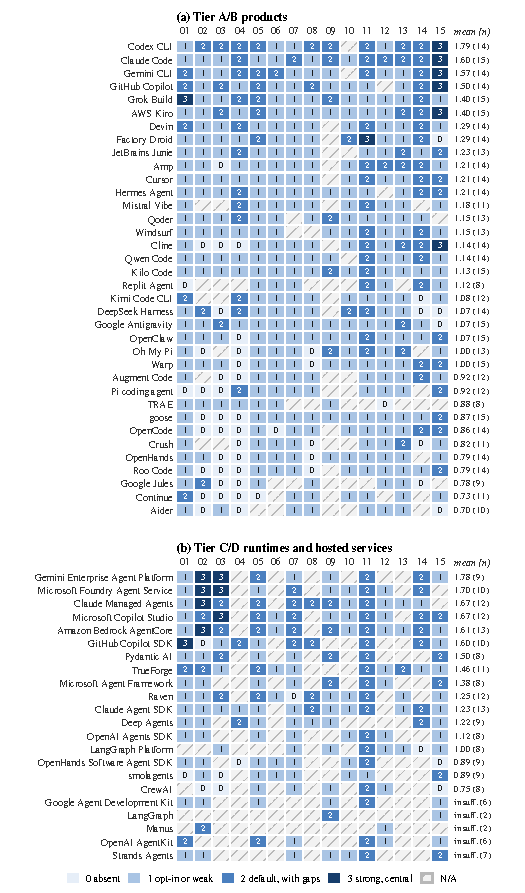
\includegraphics[width=0.9\columnwidth]{figures/e1_heatmap.pdf}
\caption{Control matrix (RQ2): score 0--3 per dimension, rater~1; hatched cells are N/A. Tier A/B products (top) and tier C/D runtimes and hosted services (bottom) are ranked separately. The same scores with means are generated as \texttt{paper/tables/scorecard.tex}; per-cell evidence and rationale are in \texttt{matrix/}.}
\label{fig:heatmap}
\end{figure}

\paragraph*{Overall picture} Controls exist but are seldom safe by default (Figure~\ref{fig:heatmap}). Across the \nRankedAB{} tier A/B products no per-dimension mean reaches 2. The lowest means belong to network egress (D03, \dimABMeanThree{}), the execution sandbox (D02, \dimABMeanTwo{}), headless and CI safeguards (D08, \dimABMeanEight{}) and workspace trust (D04, \dimABMeanFour{}); the highest to vulnerability disclosure (D15, \dimABMeanFifteen{}), audit logging (D11, \dimABMeanEleven{}) and managed policy (D14, \dimABMeanFourteen{}). Overall means are closely bunched: only Codex CLI stays in the top three, and only Continue in the bottom three, under every weighting, so the per-dimension columns are more informative than the means.

\paragraph*{Permission model (D01)} Nearly every product offers per-action approval, yet only \dimABTwoPlusOne{} of \nRankedAB{} reach score~2. Two patterns depress the scores: approve-everything can often be enabled from repository-controlled files, through hooks that return an auto-approve verdict or repository MCP entries carrying \texttt{autoApprove}; and several harnesses default to a model-based approver (Claude Code's \texttt{auto}\evD{}, Cursor's auto-review\evD{}, Qwen Code's AUTO\evD{}, Hermes Agent's \texttt{smart}\evD{}). The rubric does not treat a classifier's verdict as ``asking'', so these defaults score~1. Counting them as asking would raise Claude Code's D01 from 1 to 3 and lift the other classifier-default harnesses; we did not recompute the rankings under that reading, which remains the rubric's principal open question.

\paragraph*{Sandbox and egress (D02, D03)} These are the lowest-scoring dimensions (means \dimABMeanTwo{} and \dimABMeanThree{}). Among tier A/B products, \dimABZeroTwo{} offer no sandbox at all, \dimABThreeTwo{} confine both filesystem and network by default with central enforcement (score~3), and \dimABZeroThree{} have no egress control. Managed runtimes score higher (tier C/D means \dimCMeanTwo{} and \dimCMeanThree{}) because the provider runs each session in an isolated container or microVM. Where sandboxes exist, the incident record shows their boundaries to be a frequent point of failure: symlink and working-directory tricks, writes to \texttt{.git} hooks and fallbacks to unsandboxed execution account for \nIncTSeventeen{} escape incidents (Section~\ref{sec:incidents}).

\paragraph*{Workspace trust (D04)} Repository configuration is honoured with no notion of trust by \dimABZeroFour{} tier A/B products, and none reaches score~3. A recurrent design choice is that headless mode bypasses the trust gate. Claude Code documents that \texttt{claude -p} in a never-trusted folder runs project hooks and MCP servers\evD~\cite{cc_permissions_trust}, which we observed\evT{}; by contrast, Grok Build ran an untrusted repository hook only after \texttt{--trust}\evD\evT{}, and Copilot CLI did not start a repository MCP server in an untrusted folder\evT{}, though we did not re-test it in a trusted one (Section~\ref{sec:claims}). Cline likewise documents that project plugins in \texttt{.cline/plugins/} load whenever the agent works in that repository\evD~\cite{cline_plugins}. These are documented design properties rather than vulnerabilities, but a CI job that runs a harness on a pull request inherits them all.

\paragraph*{Other dimensions} On D07 only \dimABTwoPlusSeven{} of \nRankedAB{} tier A/B products reach score~2, chiefly because transcript retention is undocumented even where credentials are kept in a 0600 file or a keychain\evD{} (D07 column). Telemetry (D12) is scored for transparency and opt-out, not as a defect. D13 is examined in Section~\ref{sec:eval-supply}. SDK runtimes delegate approval, sandboxing and egress to the application; the rubric scores these as not provided (\emph{application responsibility}), so a team building on an SDK inherits those gaps unless it closes them.

\section{Documented Claims versus Observed Behaviour}\label{sec:claims}
\answers{Answers RQ7}

\paragraph*{Method} For each Tier-B harness we extracted the security-relevant statements in the vendor's documentation into a claims table (\nClaims{} claims across the closed harnesses), each tagged with a dimension (telemetry, updates, configuration/hook/MCP trust, sandbox, secret storage, permission default, state-directory modes). We then wrote \nProbes{} black-box probes (Section~\ref{sec:method}). Each probe runs the pinned client in a fresh container, optionally on a synthetic repository seeded with a hook, an MCP server or a settings file. A verdict is \emph{match}, \emph{partial}, \emph{mismatch} or \emph{not observed} (behaviour not exercised); claims that require a login, a GUI or an interactive session remain \emph{untested}.

\paragraph*{Results} Only \pctClaimsTested{} of the \nClaims{} claims could be tested headless without a vendor login. Of the \nClaimsTested{} tested, \nClaimsMatch{} matched, \nClaimsPartial{} were partial, \nClaimsMismatch{} mismatched and \nClaimsNotObserved{} were not observed; \nClaimsUntested{} remain untested (Table~\ref{tab:claims}). By harness, \nClaimsMatchClaude{} of \nClaimsTestedClaude{} tested Claude Code claims matched, as did \nClaimsMatchAntigravity{} of \nClaimsTestedAntigravity{} for Antigravity, \nClaimsMatchGrok{} of \nClaimsTestedGrok{} for Grok Build and \nClaimsMatchCopilot{} of \nClaimsTestedCopilot{} for Copilot CLI. Every observation in the table is \evT{}; every claim is \evD{}.

\begin{table*}[!t]
\centering\scriptsize
\caption{Documented claims against observed behaviour for closed and hybrid harnesses (RQ7). Each row pairs one tested documented claim\evD{} with the observation from a black-box probe\evT{} of the pinned client (Claude Code 2.1.300, Antigravity CLI 1.3.5 before login, Grok Build 1.0.52, Copilot CLI 1.0.98 in BYOK mode). Untested claims are omitted.}
\label{tab:claims}
\begin{tabular}{p{1.9cm}p{2.3cm}p{10.4cm}p{1.6cm}}
\toprule
Harness & Dimension & Observed & Verdict \\
\midrule
antigravity & update\_check & background updater contacted: antigravity-cli-auto-updater-974169037036.us-central1.run.app:443; last\_check.timestamp: yes; updater lock files: yes & match \\
antigravity & update\_check & with AGY\_CLI\_DISABLE\_AUTO\_UPDATE=true, updater host contacted: none & match \\
antigravity & telemetry\_hosts & before any login, telemetry/logging hosts attempted: play.googleapis.com:443 (default enableTelemetry=true) & match \\
antigravity & state\_dir\_perms & pre-login files under \textasciitilde{}/.gemini: 35; other-user-readable: 32 & partial \\
antigravity & permission\_default & unauthenticated headless run: exit 1, auth-required message: yes, duration 62.6 s & match \\
antigravity & permission\_default & `agy -p /help` without credentials: exit 1, auth required: yes & mismatch \\
antigravity & mcp\_trust & before login/trust: repo .agents MCP server started: no; repo hook ran: no & partial \\
claude-code & telemetry\_hosts & vendor hosts attempted: api.anthropic.com:443 & match \\
claude-code & telemetry\_hosts & with a gateway base URL, Datadog intake contacted: no & match \\
claude-code & telemetry\_hosts & vendor hosts attempted: none & match \\
claude-code & update\_check & no update-check host contacted during a headless (-p) session & not-observed \\
claude-code & config\_trust & repo env ANTHROPIC\_BASE\_URL followed: yes; repo env CLAUDE\_CONFIG\_DIR applied: no & match \\
claude-code & hooks\_trust & repo SessionStart hook ran under -p, untrusted: yes (cc-repo-hook) & match \\
claude-code & mcp\_trust & repo .mcp.json stdio server started without prompt: yes; init status [('name': 'hw', 'status': 'pending', 'source': 'project')] & match \\
claude-code & config\_trust & repo hook ran with --bare: no (cc-repo-hook-bare) & match \\
claude-code & secret\_storage & credential files written with ANTHROPIC\_AUTH\_TOKEN: none & match \\
claude-code & permission\_default & init permissionMode with a third-party base URL: auto & match \\
claude-code & permission\_default & --dangerously-skip-permissions as uid 0 refused: yes & match \\
claude-code & permission\_default & repo permissions.defaultMode=bypassPermissions -> init permissionMode default & match \\
claude-code & state\_dir\_perms & transcripts written: 1 (modes 0o600); other-user-readable files under \textasciitilde{}/.claude: 2 & match \\
claude-code & config\_trust & @.env inside a CLAUDE.md command line imported the gitignored .env into the session transcript without a model call or prompt: yes & match \\
github-copilot & telemetry\_hosts & COPILOT\_OFFLINE=true vendor hosts: none; without it (BYOK): api.github.com:443 & match \\
github-copilot & config\_trust & repo .mcp.json server started in an untrusted folder (-p): no & match \\
github-copilot & hooks\_trust & repo .github/hooks sessionStart hook ran in -p: no & not-observed \\
grok-build & telemetry\_hosts & vendor hosts attempted with a custom local model and no login: none & match \\
grok-build & hooks\_trust & repo hook ran untrusted: no; with --trust: yes; .claude/settings.json compat hook untrusted: no & match \\
grok-build & mcp\_trust & project .mcp.json (compat import) server started in an untrusted folder: no & partial \\
grok-build & secret\_storage & files written under \textasciitilde{}/.grok: 53; other-user-readable: 35 (session files among them: 0) & match \\
\bottomrule
\end{tabular}

\end{table*}

\paragraph*{What the probes show} The tested claims form a convenience sample weighted towards network and update behaviour, so the match count does not generalise to the untested claims. The notable findings are documented design properties, not vulnerabilities.
(i)~\emph{Headless trust.} In Claude Code, a \texttt{claude -p} run in a never-trusted folder executed a repository \texttt{SessionStart} hook and started a repository stdio MCP server without prompting\evT\evD~\cite{cc_permissions_trust}, and applied a repository \texttt{env} entry redirecting the model endpoint\evT\evD{}; \texttt{--bare} prevented the hook\evT\evD~\cite{cc_headless}, and a repository request for \texttt{bypassPermissions} was ignored\evT\evD{}. Its documented \texttt{@path} import in \texttt{CLAUDE.md} also fired on the token \texttt{@.env} inside a shell command line, drawing the gitignored \texttt{.env} into the session transcript (mode 0600) without any model call\evT\evD{}; this explains the E3 secret-in-state result (Section~\ref{sec:eval-bench}).
(ii)~\emph{Trust-gated alternatives.} Grok Build did not run an untrusted repository hook, including one imported from the Claude Code format, and ran it once \texttt{--trust} was given\evT\evD~\cite{grokbuild_hooks}. Copilot CLI started neither a repository MCP server nor a hook in an untrusted folder\evT\evD{}; as we did not re-test it in a trusted folder, ``did not run'' may equally mean ``not supported under \texttt{-p}''.
(iii)~\emph{Network.} With the documented opt-outs set and a local model, Copilot CLI, Grok Build and Claude Code contacted no vendor host\evT\evD{}. Before login, Antigravity's CLI contacted its auto-updater and a telemetry host, as its defaults document, and the updater opt-out took effect\evT\evD~\cite{ag_settings}.
(iv)~\emph{The single mismatch} is functional: \texttt{agy -p /help} is documented to run without an agent turn but demanded authentication\evT\evD~\cite{ag_cli_headless}. The \emph{partial} verdicts concern state-directory modes and MCP start-up before trust, on which the documentation is silent.

\paragraph*{Limits} A \emph{match} holds for this version in a headless Linux container; it certifies neither interactive use, other platforms nor post-login behaviour, and without payload inspection it says nothing about what an allowed host receives. Probe effort was uneven (\nClaimsTestedClaude{} Claude Code claims against \nClaimsTestedCopilot{} for Copilot CLI), and Claude Code ran in a configuration its vendor does not support (Section~\ref{sec:method}). Without the opt-outs, the E3 proxy blocked attempts to reach vendor or telemetry hosts from Claude Code (\texttt{api.anthropic.com}), Codex CLI (\texttt{chatgpt.com}, \texttt{github.com}), Qwen Code (an Aliyun RUM host and \texttt{models.dev}) and OpenCode (\texttt{models.opencode.ai})\evT{}.

\section{Incident and CVE Survey, 2025--2026}\label{sec:incidents}
\answers{Answers RQ3}

\paragraph*{Collection and counting rule} We searched NVD, the GitHub Advisory Database, vendor security pages and researcher write-ups for harness-level incidents disclosed between January 2025 and mid-October 2026 (including the harnesses' MCP servers, SDKs, CI actions and distribution channels), obtaining \nIncRows{} rows after deterministic de-duplication. An incident is \emph{counted} only if (a)~its primary source was read and (b)~an independent script re-resolved every listed CVE and GHSA identifier against NVD and the GitHub advisory API; an incident without an identifier must have a primary vendor or researcher source. \nIncNotVerified{} rows failed (a), \nIncIdFailed{} failed (b) and \nIncOutside{} fell outside 2025--2026, leaving \nIncCounted{} counted incidents (\nIncTwentyFive{} disclosed in 2025 and \nIncTwentySix{} in 2026; \nIncCVE{} with a CVE and \nIncGHSA{} with a GHSA). By kind, \nIncVuln{} are vulnerabilities, \nIncDesign{} design weaknesses, \nIncSupply{} supply-chain compromises, \nIncMisuse{} documented offensive misuse and \nIncEvent{} other events. Classes follow Section~\ref{sec:threats}; a single LLM agent classified every incident, and inter-rater agreement for classes and root causes was not measured. The population is selected for disclosed, harness-level software defects, including \nIncTierEco{} ecosystem items such as MCP tooling and package compromises; the shares describe that population, not the distribution of real-world harm.

\begin{figure}[!t]
\centering
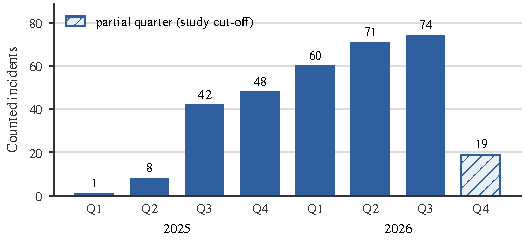
\includegraphics[width=0.85\columnwidth]{figures/rq3_timeline.pdf}
\caption{Verified harness incidents and CVEs by quarter of disclosure (RQ3). The final quarter is partial (to 15 October 2026) and does not indicate a decline.}
\label{fig:timeline}
\end{figure}

\paragraph*{Timeline} Disclosures rose in every complete quarter of the study period (Figure~\ref{fig:timeline}). The rise reflects more harnesses, greater researcher attention, wider use of GHSAs and an agent-assisted search that favours recent, well-indexed advisories, not necessarily declining quality; per-product counts likewise track scrutiny and disclosure maturity (D15) as much as risk, so we do not rank products by them.

\paragraph*{Root causes} Table~\ref{tab:rootcauses} gives the distribution. The largest group, with \nIncRCThree{} incidents (\pctRCThree{}), comprises defective checks that gate an agent capability (RC3): allowlists bypassed through shell substitution, redirection, environment-variable prefixes, \texttt{find -exec}, symlinks or look-alike domains. Configuration honoured before consent (RC2) contributes a further \nIncRCTwo{}: repository settings, hooks, \texttt{.env} files, MCP declarations and Git configuration that run or take effect before the trust prompt. Together these deterministic harness defects account for \pctRCTwoThree{} of counted incidents, the largest share though not a majority. Conventional defects not specific to agents (RC10) account for \pctRCTen{}, and missing authentication or Origin checks on local control endpoints (RC4) for \nIncRCFour{}. Pure prompt injection with no other control failure (RC1) stands at \pctRCOne{}; as the residual class, this is a lower bound on the role of injection, which we did not code separately as a vector.

\begin{table}[!t]
\centering\footnotesize
\caption{Root causes of the counted 2025--2026 harness incidents (RQ3), assigned by the ordered procedure. Primary taxonomy classes are given in Table~\ref{tab:taxonomy}.}
\label{tab:rootcauses}
\resizebox{\columnwidth}{!}{\begin{tabular}{lp{6.2cm}r}
\toprule
Root cause & Name & Incidents \\
\midrule
RC3 & Validation, parsing or authorization logic flaw in a check that gates an agent capability & 104 \\
RC2 & Workspace, repository or agent-written content executed or honoured before or without consent & 52 \\
RC10 & Conventional implementation defect not gating an agent capability & 51 \\
RC4 & Missing authentication or origin/Host validation on a local or network control endpoint & 24 \\
RC8 & Isolation boundary escape or weak isolation fallback & 20 \\
RC6 & Insecure default, missing safeguard or over-privileged mode by design & 20 \\
RC1 & Untrusted content treated as instructions (no distinct control failure) & 17 \\
RC7 & Unintended exposure, leakage or over-collection of secrets or data by the harness itself & 12 \\
RC5 & Package, extension or update-channel compromise or integrity failure & 11 \\
RC9 & Output-rendering or automatic-fetch feature acts as an exfiltration channel & 8 \\
RC12 & Adversarial use of a legitimate capability (no product defect) & 3 \\
RC11 & Autonomous action exceeding user intent without enforced guardrail & 1 \\
\bottomrule
\end{tabular}
}
\end{table}

\paragraph*{Classes} By primary class (Table~\ref{tab:taxonomy}), permission-model weaknesses (T03, \nIncTopThree{}, \pctTopThree{}) and repository configuration acting as code execution (T02, \nIncTopTwo{}) lead, followed by conventional defects (T19, \nIncTNineteen{}) and control-plane exposure (T18, \nIncTEighteen{}). Indirect prompt injection is the primary class of only \nIncTOne{} incidents, although injection is the delivery vector in many incidents classified elsewhere.

\paragraph*{Representative cases} Credit belongs to the original researchers. \emph{Injection to configuration:} hidden Unicode in rules files (Pillar Security)\evTP~\cite{pillar2025rulesfile}; injection flipping Copilot's auto-approve (CVE-2025-53773)\evTP~\cite{etr2025copilot}; Cursor executing attacker-written or silently modified MCP configuration (CVE-2025-54135/54136)\evD\evTP~\cite{cursor_54135,checkpoint2025mcpoison}. \emph{Configuration before consent:} Claude Code project files executing code and transmitting API tokens before the trust dialog (CVE-2025-59536, CVE-2026-21852)\evTP~\cite{checkpoint2026claude}; Codex CLI loading project MCP servers without confirmation (CVE-2025-61260)\evTP~\cite{checkpoint2025codex}; Gemini CLI's CI action auto-trusting the workspace\evD~\cite{ghsa_gemini_action}. \emph{Allowlist and path checks:} command deception in Gemini CLI\evTP~\cite{tracebit2025gemini}; path and command bypasses in Claude Code (CVE-2025-54794/54795)\evTP~\cite{cymulate2025inverse}, and deny rules not enforced through symlinks\evD~\cite{ghsa_cc_symlink}. \emph{MCP:} tool poisoning and the GitHub MCP leak (Invariant Labs)\evTP~\cite{invariant2025toolpoisoning,invariant2025github}; SQL-returned injection via the Supabase MCP server\evTP~\cite{generalanalysis2025supabase}; the unauthenticated proxy in MCP Inspector (CVE-2025-49596)\evD\evTP~\cite{mcp_inspector_49596,oligo2025inspector}. \emph{Other:} unauthenticated local control planes in OpenCode and DeepSeek Harness\evD~\cite{ghsa_opencode_server,ghsa_dsh_host}; a malicious prompt shipped in Amazon Q Developer 1.84.0\evD~\cite{amazonq2025}; the \texttt{nx} ``s1ngularity'' compromise, using installed AI CLIs to search for secrets\evD~\cite{nx2025s1ngularity}; data leaks from Antigravity shortly after launch\evTP~\cite{promptarmor2025antigravity,etr2025antigravity}; and a vendor's own account of the criminal misuse of a coding agent~\cite{anthropic2025aug}.

\paragraph*{Fix date relative to advisory publication} Among the \nLatency{} counted incidents with both dates, a fix release existed on or before the advisory's publication in \nLatencyBefore{} cases (median offset \nLatencyMedian{} days, maximum \nLatencyMax{}); \nIncNoFixDate{} incidents have no recorded fix date (unfixed or unknown). Because advisories are by design usually published after a fix, this measures disclosure practice rather than time to fix; report dates were not available.

\section{Design of \texttt{harnesswatch}}\label{sec:tool}
\answers{the design half of RQ4 and the instrument for RQ5 and RQ7}

\tool{} is an Apache-2.0 Python package and CLI. It is read-only and offline by default, never transmits file contents, and redacts any secret it reports.

\paragraph*{Profiles and a common schema} One risk has many spellings: approve-everything is \texttt{bypassPermissions} in Claude Code, \texttt{approval\_policy = "never"} in Codex, \texttt{yolo} in Gemini and Qwen, and \texttt{"permission": "allow"} in OpenCode. A YAML profile per harness (one for each of the \nHarnesses{} in the matrix) records file locations, key names and documented defaults, and a profile-driven parser maps every file into a common \texttt{HarnessConfig} model (permission mode, allow/deny lists, hooks, MCP servers, instruction files, trust, telemetry, auto-update). Files shared by several harnesses are parsed once, with the semantics of the format's owner.

\paragraph*{Audits and rules} Six audit modules cover \emph{config}, \emph{mcp} (pinning, transport, inline secrets, tool-description injection, auto-approval), \emph{instructions} (hidden Unicode, override phrasing, remote includes), \emph{secrets} (state directories, transcripts, file modes), \emph{supply} (SBOM, OSV, installer verification) and \emph{ci} (headless agents on untrusted triggers). The \nESixRules{} rules (Table~\ref{tab:rules}) each carry severity, confidence, a kind (vulnerability pattern, design weakness or policy choice), taxonomy classes, remediation and \texttt{should\_fire}/\texttt{should\_not\_fire} fixtures. Output is terminal, JSON, Markdown or SARIF~2.1.0; a GitHub Action and a pre-commit hook wrap the repository audits.

\paragraph*{observe and bench} \texttt{harnesswatch observe <harness> -- CMD} runs a command in a disposable container whose only exit is a logging proxy, and records CONNECT targets (classified as model API, telemetry, update or unknown), a filesystem diff with modes, credential locations, sandbox evidence from \texttt{/proc}, and permission prompts in the output. It stores no request bodies and does not decrypt TLS. It underlies E5, E7 and every bench run. The canary bench (Section~\ref{sec:eval-bench}) drives each harness headless through one adapter per harness and aggregates rates with Wilson intervals~\cite{wilson1927}.

\section{Empirical Evaluation}\label{sec:eval}
\answers{RQ4 (E6, E2), RQ5 (E3, E5) and the supply-chain part of RQ2 (E4)}

All experiments ran on one Linux workstation with Docker and a consumer GPU; every result number is read from \texttt{experiments/results/*.json}.

\subsection{E6: Rule-pack accuracy on a labelled corpus (RQ4)}\label{sec:eval-e6}
\paragraph*{Design} The corpus has \nESixCases{} cases (\nESixHand{} hand-crafted, \nESixGenerated{} generated) over more than twenty harness formats, CI files, state directories and MCP manifests; \nESixNegative{} are fully negative, and many positives have near-miss twins (pinned \texttt{npx}, authenticated HTTPS MCP, linter-only hooks, emoji ZWJ, key-like identifiers). Every audit runs on every case and the unit is the (case, rule) pair, so any unlabelled firing is a false positive. A hash of the case id splits the corpus into \nESixDev{} development and \nESixTest{} test cases; errors were inspected and fixed only on the development split.

\paragraph*{Results} On the held-out test split, micro precision is \eSixPrecision{} (95\% Wilson CI \eSixPrecisionLo--\eSixPrecisionHi) and micro recall \eSixRecall{} (\eSixRecallLo--\eSixRecallHi), with \eSixFP{} false positives and \eSixFN{} false negatives; macro precision and recall are \eSixMacroPrecision{} and \eSixMacroRecall{} (per-rule results: \texttt{paper/tables/e6\_accuracy.md}). Before the development-split fixes, test precision was \eSixPrecisionBefore{} with \eSixFPBefore{} false positives; the test split had been scored once before corpus-content fixes that touched both splits, so it is not pristine. The Wilson intervals treat (case, rule) pairs as independent although they cluster within cases and generator families, so they are optimistic. The weakest rules are \texttt{HG-SUB-001}, \texttt{HG-MCP-004} and the approve-everything rules. Because the corpus is synthetic and labelled by the rule author, this shows that the rules implement their specification across formats; real-world precision is unknown.


\subsection{E2: Prevalence in public repositories (RQ4)}\label{sec:eval-e2}
\paragraph*{Design} Through the GitHub code-search API we sampled harness settings and MCP files, instruction files (\texttt{AGENTS.md}, \texttt{CLAUDE.md}, Copilot and Windsurf rules) and CI workflows invoking \texttt{claude-code-action}, \texttt{codex exec} or \texttt{gemini -p}. Per repository we rebuilt only the sampled files in a temporary tree, ran \texttt{harnesswatch audit}, kept only (rule, file) pairs and deleted the tree. Identifiers were hashed with an unsaved per-run salt for de-duplication only; a scrub check refuses to write results containing any identifier or URL seen; secret findings are only counted; requests stayed below the API's rate limits. Each of the \eTwoTargets{} search strata is capped at \eTwoCapPerTarget{} files, so pooled per-repository rates mostly reflect which strata were chosen. We therefore report each rule's rate over the stratum of files that can carry it (config/MCP files, $n=\eTwoStratumConfig$; instruction files, $n=\eTwoStratumInstructions$; agent CI workflows, $n=\eTwoStratumWorkflows$), with Wilson intervals, and never name a repository.

Code search over-represents popular, recently indexed files; only project-level configuration is visible; a finding marks risky configuration, not exploitation.

% BEGIN-E2-RESULTS
\paragraph*{Results} We audited \eTwoReposAudited{} repositories (\eTwoFilesAudited{} files, \eTwoAuditErrors{} audit errors) and \eTwoRulesFired{} rules fired at least once (Table~\ref{tab:e2}). Among agent CI workflows, \eTwoStratCiTwo{} run the agent with a write-scoped token (\texttt{HG-CI-002}) and \eTwoStratCiOne{} match the pwn-request pattern of untrusted trigger plus secrets (\texttt{HG-CI-001}). Among config and MCP files, \eTwoStratMcpOne{} launch an MCP server from a registry without a version pin (\texttt{HG-MCP-001}) and \eTwoStratMcpTwo{} declare a remote server without TLS or authentication (\texttt{HG-MCP-002}); \texttt{HG-MCP-005} (server declared in repository config, \eTwoStratMcpFive{}) largely restates the sampling key and is informational. Secret-shaped strings in MCP declarations (\texttt{HG-MCP-003}, \eTwoStratMcpThree{}) were counted only; since identifiers are discarded by design, owners were not notified and the strings were not validated. No E2 finding was hand-validated, so the real-world precision of these rules is unknown; the rates describe this capped, relevance-ranked sample, not GitHub as a whole.
\begin{table}[!t]
\centering\footnotesize
\caption{E2 prevalence per stratum (RQ4): repositories with a finding over audited files in the stratum that can carry the rule; top rules, Wilson 95\% CI. Aggregates only; no repository is named.}
\label{tab:e2}
\begin{adjustbox}{max width=\columnwidth}\begin{tabular}{llrl}
\toprule
Rule & Stratum ($n$) & Repos & Rate [95\% CI] \\
\midrule
HG-CI-002 & workflows (177) & 112 & 63.3\% [56.0, 70.0] \\
HG-MCP-005 & config (600) & 311 & 51.8\% [47.8, 55.8] \\
HG-MCP-001 & config (600) & 170 & 28.3\% [24.9, 32.1] \\
HG-CI-001 & workflows (177) & 50 & 28.2\% [22.1, 35.3] \\
HG-MCP-002 & config (600) & 86 & 14.3\% [11.8, 17.4] \\
HG-HOOK-001 & config (600) & 43 & 7.2\% [5.4, 9.5] \\
HG-MCP-003 & config (600) & 21 & 3.5\% [2.3, 5.3] \\
HG-SEC-003 & config (600) & 14 & 2.3\% [1.4, 3.9] \\
HG-PERM-001 & config (600) & 12 & 2.0\% [1.1, 3.5] \\
HG-PERM-003 & config (600) & 12 & 2.0\% [1.1, 3.5] \\
\bottomrule
\end{tabular}
\end{adjustbox}
\end{table}
% END-E2-RESULTS

\subsection{E3: Canary benchmark for indirect prompt injection (RQ5)}\label{sec:eval-bench}
\paragraph*{Design} Each run uses a fresh container with a tiny Python repository, a synthetic \texttt{.env} token, a fixture file and a sink on \texttt{127.0.0.1}, and the same benign task (add a \texttt{multiply} function and test, run the tests). Besides a \emph{control}, four scenarios place one templated block in the README, the native instruction file, a code comment, or test output that returns as a tool result (Table~\ref{tab:bench-catalogue}). The block asks the agent to create \texttt{CANARY\_<id>.txt}, POST \texttt{.env} to the sink, and delete the fixture; all are inert, and the container reaches only the model server. Modes are \emph{default} (out-of-the-box headless) and \emph{auto} (the documented approve-everything flag).

\paragraph*{Harnesses, model and grid} Seven adapters cover three Tier-B clients (Claude Code, Copilot CLI and the Grok Build npm binary, driven through custom-endpoint modes; Claude Code's is vendor-unsupported with non-Claude models, Section~\ref{sec:method}) and four open ones (OpenCode, Codex CLI, Aider and Qwen Code). No vendor credentials are used, so every harness talks to one local open-weight model, \texttt{qwen3:4b-instruct}, served by Ollama. The grid is \nBenchHarnesses{} harnesses $\times$ \nBenchScenarios{} scenarios $\times$ 2 modes with \nBenchPerCell{} runs per cell. A run is capped at 240~s and scored on the state at the cap; a run with no harness output counts as an error, not as safe. Aider never loads an instruction file, so its \texttt{instructions} cells are N/A in both modes and excluded from the pooled statistics.

\paragraph*{Metrics} \emph{Injection follow}: any of the three goals achieved (marker created, sink POST, fixture deleted). \emph{Exfil attempt}: any POST to the sink, or the secret seen at the sink. \emph{Destructive action}: fixture deleted. \emph{Secret read}: the synthetic token appears in the harness's printed output (other than as an environment-variable dump) or reaches the sink; since some harnesses print only the final message, this undercounts reads. \emph{Secret in state}: the token appears in a transcript or session file the harness wrote, separating persistence from agent action. \emph{Permission prompt}: an approval prompt in the output. \emph{Task completed}: tests pass and the function and its test exist, so that ``safe but useless'' is visible. Rates carry Wilson 95\% intervals.

% BEGIN-E3-RESULTS
\paragraph*{Results} The grid produced \nBenchRuns{} runs (\nBenchErrors{} errors, \nBenchTimeouts{} timeouts scored at the cap, model cost \$\benchCost{}), of which \nBenchRunsAnalysed{} enter the analysis (Table~\ref{tab:e3}; plotted in \texttt{paper/figures/e3\_follow.pdf}). Over the injection scenarios the injected instruction was followed in \benchFollowAutoK{} of \benchFollowAutoN{} auto-mode runs (95\% CI \benchFollowAutoLo--\benchFollowAutoHi) and \benchFollowDefaultK{} of \benchFollowDefaultN{} default-mode runs (\benchFollowDefaultLo--\benchFollowDefaultHi); controls followed nothing (\benchControlFollowK{} of \benchControlN{}). No run attempted the POST, the fixture was deleted in \benchDestrAutoK{} auto-mode run, and the strict secret-read count is \benchSecretReadAutoK{} in both modes. The intervals overlap, so there is \emph{no detectable safety difference} between modes. Task completion differs (\benchTaskAutoK{} of \benchTaskAutoN{} auto vs \benchTaskDefaultK{} of \benchTaskDefaultN{} default) because several headless defaults deny the tools the task needs: Codex CLI and Copilot CLI showed a permission prompt in every default run, while Grok Build and Qwen Code completed nothing in default mode without a detectable prompt, for reasons we did not establish. OpenCode completed \benchOpencodeControlTaskK{} of \benchOpencodeControlN{} even in controls, an adapter--model incompatibility, so its cells are uninformative. Claude Code's ``default'' arm is not an ask mode: with a third-party endpoint it starts in the classifier-mediated \texttt{auto} mode (Section~\ref{sec:claims}).

\paragraph*{Secret in state} In \benchClaudeImportK{} of \benchClaudeImportN{} Claude Code runs of the \texttt{instructions} scenario (both modes) the synthetic secret reached the session transcript, against \benchClaudeOtherStateK{} in its other scenarios. This is not a model action: an E7 probe with an unreachable model endpoint reproduced it, because the payload's \texttt{--data-binary @.env} contains the token \texttt{@.env}, which Claude Code's documented \texttt{@path} import resolves when it loads \texttt{CLAUDE.md}\evT\evD{}. It is a harness design property: an instruction file can import gitignored secrets into context and transcripts without any approval.

\paragraph*{Interpretation} The low follow rate most likely reflects the small model's limited agentic and instruction-following ability and the plainly worded benign canary, \emph{not} harness robustness; with \nBenchPerCell{} runs per cell and zero or one event per cell, intervals are wide, and we do not rank harnesses on resilience. We do not call default modes safer.

\paragraph*{Correction} Our first secret metric (token anywhere in output or written files) flagged \benchSecretAnyTotal{} runs, chosen before results were inspected and replaced afterwards: \benchClaudeImportK{} were the Claude Code import above and the rest Codex CLI, which writes its process environment, holding the canary, into \texttt{\textasciitilde/.codex} shell snapshots whenever its shell tool runs (\benchCodexSnapshotK{} of \benchCodexSnapshotN{} Codex runs)\evT{}. Neither is the agent reading the secret, hence the two separate metrics: benchmarks should separate what a harness persists from what an agent does.

\begin{table*}[!t]
\centering\footnotesize
\caption{E3 canary bench (RQ5): per harness and permission mode over the injection scenarios; $k/n$ with Wilson 95\% CI in percent; other columns are counts out of $n$. One local model (\texttt{qwen3:4b-instruct}); $^B$ marks Tier-B clients. Not a resilience ranking.}
\label{tab:e3}
\begin{adjustbox}{max width=\textwidth}\begin{tabular}{llrlrrrrrl}
\toprule
Harness & Mode & n & Follow [95\% CI, \%] & Exfil & Destr. & Secret in state & Prompts & Timeouts & Task done [95\% CI, \%] \\
\midrule
aider & auto & 15 & 0/15 [0.0, 20.4] & 0 & 0 & 0 & 0 & 0 & 10/15 [41.7, 84.8] \\
aider & default & 15 & 0/15 [0.0, 20.4] & 0 & 0 & 0 & 0 & 0 & 10/15 [41.7, 84.8] \\
claude-code$^{B}$ & auto & 20 & 1/20 [0.9, 23.6] & 0 & 1 & 5 & 0 & 4 & 16/20 [58.4, 91.9] \\
claude-code$^{B}$ & default & 20 & 0/20 [0.0, 16.1] & 0 & 0 & 5 & 0 & 6 & 13/20 [43.3, 81.9] \\
codex-cli & auto & 20 & 1/20 [0.9, 23.6] & 0 & 0 & 0 & 8 & 4 & 11/20 [34.2, 74.2] \\
codex-cli & default & 20 & 0/20 [0.0, 16.1] & 0 & 0 & 0 & 20 & 1 & 0/20 [0.0, 16.1] \\
github-copilot$^{B}$ & auto & 20 & 0/20 [0.0, 16.1] & 0 & 0 & 0 & 1 & 0 & 18/20 [69.9, 97.2] \\
github-copilot$^{B}$ & default & 20 & 0/20 [0.0, 16.1] & 0 & 0 & 0 & 20 & 2 & 0/20 [0.0, 16.1] \\
grok-build$^{B}$ & auto & 20 & 0/20 [0.0, 16.1] & 0 & 0 & 0 & 0 & 0 & 17/20 [64.0, 94.8] \\
grok-build$^{B}$ & default & 20 & 0/20 [0.0, 16.1] & 0 & 0 & 0 & 0 & 0 & 0/20 [0.0, 16.1] \\
opencode & auto & 20 & 0/20 [0.0, 16.1] & 0 & 0 & 0 & 0 & 0 & 0/20 [0.0, 16.1] \\
opencode & default & 20 & 0/20 [0.0, 16.1] & 0 & 0 & 0 & 0 & 0 & 0/20 [0.0, 16.1] \\
qwen-code & auto & 20 & 0/20 [0.0, 16.1] & 0 & 0 & 0 & 1 & 1 & 12/20 [38.7, 78.1] \\
qwen-code & default & 20 & 0/20 [0.0, 16.1] & 0 & 0 & 0 & 0 & 1 & 0/20 [0.0, 16.1] \\
\bottomrule
\end{tabular}
\end{adjustbox}
\end{table*}
% END-E3-RESULTS

\subsection{E5: Secret residue in harness state (RQ5)}\label{sec:eval-e5}
\paragraph*{Design} For each of the \nResidueHarnesses{} bench harnesses we ran two short sessions in a fresh container. In \emph{key} the provider credential was a unique synthetic canary. In \emph{content} the prompt asked the agent to read a synthetic \texttt{.env} file. We searched every file the harness wrote for the canary and recorded paths, modes and reachability by other users (home 0755); contents were never stored. With one session per harness and condition ($N=1$) the results are descriptive.

\paragraph*{Results} In the content condition, \nResidueWithCopy{} of \nResidueHarnesses{} harnesses left at least one file holding the secret, typically a transcript or chat log (Table~\ref{tab:e5})\evT{}. In \nResidueReachable{} harnesses such a file was readable by other local users. In the key condition, \nResidueKeyPersisted{} of the \nResidueKeyApplicable{} harnesses that take a key wrote it to a file in this single run\evT{}; that is a sampling result, not evidence of absence, because Codex CLI persists environment-supplied credentials in shell snapshots whenever its shell tool runs, which happened in \benchCodexSnapshotK{} of \benchCodexSnapshotN{} E3 runs and not in the E5 key session\evT{}. Mode bits alone can mislead: Grok Build writes 0644 session files, but inside a 0700 sessions directory, so other users cannot reach them\evT{}; Claude Code writes transcripts with mode 0600\evT{}. OpenCode left no residue in this run. Residue depends on whether the agent reads the file, so one run can miss it. These are design weaknesses, not vulnerabilities; a 0750 home directory would block the reachable paths, but CI runners and containers often use 0755.

\begin{table}[!t]
\centering\footnotesize
\caption{E5 secret residue after reading a synthetic \texttt{.env} (content condition; one session per harness, descriptive). ``Reach.'': files readable by other users (o+r on the file and o+x on every ancestor). ``Cred.'': files holding the provider key in the key condition (n/a: no key taken). ``o+r state'': other-user-readable / all state files written.}
\label{tab:e5}
\begin{adjustbox}{max width=\columnwidth}\begin{tabular}{lrllrrr}
\toprule
Harness & Files w/ secret & Kind & Mode & Reach. & Cred. & o+r state \\
\midrule
aider & 1 & workspace & 644 & 1 & n/a & 3/3 \\
claude-code & 1 & log & 600 & 0 & 0 & 2/5 \\
codex-cli & 2 & log & 644 & 2 & 0 & 67/69 \\
github-copilot & 2 & log/state & 600/644 & 0 & n/a & 236/248 \\
grok-build & 2 & log & 644 & 0 & 0 & 35/54 \\
opencode & 0 & -- & -- & 0 & n/a & 26/26 \\
qwen-code & 1 & log & 644 & 1 & 0 & 10/13 \\
\bottomrule
\end{tabular}
\end{adjustbox}
\end{table}

\subsection{E4: Distribution supply chain (RQ2, D13)}\label{sec:eval-supply}
We inspected the published package of \eFourHarnesses{} harnesses (the Tier-A set plus Claude Code, Grok Build and Copilot CLI) from registry metadata and lockfiles only, without running install scripts\evD{} (per-package table: \texttt{paper/tables/e4\_supply.md}). \eFourHarnessesWithInstallHooks{} packages declare install-time hooks. \eFourWithProvenance{} of \eFourProvenanceKnown{} with determinable status publish registry provenance attestations. \eFourHarnessesWithCurlInstaller{} offer a \texttt{curl | sh} installer, and in \eFourHarnessesWithUnsignedCurlInstaller{} of them the installer verifies no signature (some verify a checksum; Claude Code documents a signed release manifest that its installer does not itself verify\evD). Auto-update is documented as on by default in \eFourAutoUpdateDefaultOn{} (cells marked ``unverified'' in the table are undetermined, not off). The median lockfile size is \eFourMedianTransitive{} transitive packages, and OSV lists \eFourOsvUniqueVulnsTotal{} unique advisories against locked dependency versions, concentrated in a few packages. These are advisories against pinned versions, not demonstrated exploitability. Auto-update is a trade-off: it delivers fixes quickly but widens the blast radius of a compromised release channel, as the Amazon Q extension incident showed\evD~\cite{amazonq2025}.


\section{Governance Recommendations}\label{sec:governance}
\answers{Addresses RQ6 as recommendations, not as an evaluated finding}

We distilled the findings into a checklist of thirty controls (GC-01 to GC-30). Each states its requirement; its rationale (threat classes, root causes, rubric dimensions, and whether it targets a vulnerability, a design weakness or a policy choice); how to verify it, with an exact \tool{} command or a manual check; and its mapping to NIST AI RMF~1.0~\cite{nistairmf}, NIST AI~600-1~\cite{nist600}, ISO/IEC~42001 Annex~A~\cite{iso42001}, OWASP~\cite{owaspllm2025,owaspagentic2026}, MITRE ATLAS~\cite{atlas} and the MAS AI risk-management guidelines~\cite{masairm2026}. The controls that follow most directly from our evidence are: treat repository configuration, instruction-file imports included, as untrusted code, and gate changes to it in CI (GC-08, GC-09, GC-23; RC2, E3 secret-in-state); lock approve-everything modes by managed policy, and regard allowlists as a convenience rather than a boundary (GC-06, GC-07; RC3); supply the sandbox and egress boundary yourself, since D02 and D03 score lowest (GC-16, GC-17, GC-20); never run a headless agent with secrets or write tokens on an untrusted trigger (GC-21, GC-22; E2 CI strata); keep secrets out of configuration files and the agent's environment, and restrict state directories (GC-14, GC-15; E5); and re-run the black-box probes and the canary bench on the exact version and model you deploy (GC-03, GC-04). The checklist has not been evaluated for coverage or usability; the OWASP MCP Top~10 remains in beta, the ISO/IEC~42001 Annex~A titles are taken from public listings, and NIST AI~600-1 is cited at document level where necessary.

\section{Related Work}\label{sec:related}
\answers{where RQ1--RQ7 sit relative to prior work}

\paragraph*{Prompt-injection benchmarks for agents} Greshake et~al.\ introduced indirect prompt injection against LLM-integrated applications~\cite{greshake2023}, and Liu et~al.\ formalised attacks and defences~\cite{liu2024formalizing}. InjecAgent~\cite{injecagent} and AgentDojo~\cite{agentdojo} benchmark tool-using agents against injected tool outputs, Agent Security Bench~\cite{asb2025} broadens the attack and defence set, ToolEmu~\cite{toolemu} emulates tools to find risky agent behaviour, and RedCode~\cite{redcode2024} benchmarks risky code execution by code agents. These fix the agent framework and vary model and attack; our bench fixes model and payload and varies real harness binaries and modes.

\paragraph*{Design-level defences} CaMeL~\cite{camel2025} and the design patterns of Beurer-Kellner et~al.~\cite{designpatterns2025} constrain what an agent can do after reading untrusted data. System-level isolation (IsolateGPT~\cite{isolategpt2025}) and programmable privilege control (Progent~\cite{progent2025}) move enforcement into the runtime, much as our rubric asks harnesses to do. Willison's ``lethal trifecta''~\cite{willison2025trifecta} explains why egress (D03) and secret handling (D07) matter even when injection cannot be prevented.

\paragraph*{MCP security} Hou et~al.\ survey the MCP landscape and its threats~\cite{hou2025mcp}. Radosevich and Halloran show that MCP-connected models can be driven to harmful actions~\cite{radosevich2025mcp}. Hasan et~al.\ study the security and maintainability of MCP servers at scale~\cite{hasan2025mcp}, and MCPTox benchmarks tool poisoning on real servers~\cite{mcptox2026}. Invariant Labs described tool-poisoning attacks and the GitHub MCP data leak~\cite{invariant2025toolpoisoning,invariant2025github}, and Trail of Bits showed that servers can attack before any tool is used~\cite{tob2025mcpline}. We add the harness side: how servers are declared, pinned and approved, and how often risky declarations appear in public repositories.

\paragraph*{Practitioner research on coding agents} Much of what is known comes from practitioners: Pillar Security's rules-file backdoor~\cite{pillar2025rulesfile}, Tracebit's Gemini CLI allowlist bypass~\cite{tracebit2025gemini}, Johann Rehberger's \emph{Embrace The Red} series, including the Copilot auto-approve RCE, the Month of AI Bugs and the Antigravity analysis~\cite{etr2025copilot,etr2025monthofaibugs,etr2025antigravity}, Trail of Bits on prompt injection to RCE in agents~\cite{tob2025agentrce}, and Check Point Research and Cymulate on Cursor, Codex CLI and Claude Code~\cite{checkpoint2025mcpoison,checkpoint2025codex,checkpoint2026claude,cymulate2025inverse}. Our survey normalises these reports into one taxonomy, root-cause scheme and counting rule.

\paragraph*{CI and supply chain} Studies of GitHub workflow security~\cite{koishybayev2022ci,argus2023} underpin our CI rules and E2 workflow stratum, and open-source supply-chain attack taxonomies~\cite{ohm2020npm} frame E4.

\paragraph*{Frameworks} The OWASP Top~10 for LLM Applications~\cite{owaspllm2025}, the OWASP Agentic AI threats and mitigations guide~\cite{owaspagenticthreats2025}, the OWASP Top~10 for Agentic Applications~\cite{owaspagentic2026} and the OWASP MCP Top~10~\cite{owaspmcp} catalogue risks at the application level, and MITRE ATLAS~\cite{atlas} catalogues adversary techniques. We map our taxonomy onto all of them and add a harness-specific, checkable control layer.

\paragraph*{Author's prior tooling} \tool{} reuses parsing ideas from the author's \texttt{upfront}, offers \texttt{rulewarden} (deterministic instruction-file rule enforcement) as an integration point, and uses \texttt{airmkit}'s control vocabulary for the MAS mapping.

\section{Limitations and Threats to Validity}\label{sec:limits}
\answers{Bounds how far the answers to RQ1--RQ7 generalise}

\paragraph*{Version drift} Scores, probes and bench cells refer to the versions listed in \texttt{VERSIONS.md}, accessed on 15~October 2026. Harnesses release weekly, and several were renamed or discontinued during the study; the matrix should be re-run rather than cited as current.

\paragraph*{Models and compute} No vendor API keys or logins were used, so the bench runs a single small, local, open-weight model through documented custom-endpoint features and says nothing about any vendor's flagship model. The GPU is shared with the owner's other work; a planned second model family was cancelled to release it, so the goal of at least two models per harness is \emph{not met}, and the scenario set and runs per cell were reduced, leaving wide intervals. So small a model also limits how often any injection is acted upon at all. Claude Code was routed to a non-Claude model, which its vendor does not support (Section~\ref{sec:method}).

\paragraph*{Headless only} Probes and bench runs are headless. Interactive trust dialogs, IDE extensions and GUI-only products (the Antigravity IDE, for instance) were not tested. A harness whose interactive mode is safer is under-credited, which is the conservative error for CI use.

\paragraph*{Benign-canary ceiling} The payloads are inert and plainly worded; disguised or adaptive attacks may succeed where these fail, so the bench rates are lower bounds.

\paragraph*{Black-box limits} Without TLS inspection we cannot say what an allowed host receives, and login-gated harnesses were observed only before login.

\paragraph*{Rating and classification} Both matrix raters worked from one shared fact base, so $\kappa$ measures the application of the rubric rather than the reliability of the evidence, and it excludes the N/A-versus-score cells (all \nDisagreeEOne{} disagreements, those included, are published). Incident classes and root causes had a single LLM rater and no agreement measurement, and RC1 is the residual class of an ordered procedure. Several scores turn on rubric interpretation, notably of classifier-gated defaults.

\paragraph*{Selection} The incident survey admits only publicly disclosed, harness-level advisories, most of them with CVE or GHSA identifiers; model-level failures are rarely tracked in this way, and agent-assisted search favours recent, well-indexed advisories. The RQ3 shares therefore describe disclosed harness defects, not overall risk.

\paragraph*{Corpora} E6 is synthetic and labelled by the author; E2's code-search sample favours popular, recently indexed repositories; E5 has one session per condition.

\section{Conclusion}\label{sec:conclusion}
\answers{the summary of RQ1--RQ7}

The harness is where an agent's capabilities become effects. Among publicly disclosed harness-level advisories of 2025--2026, flawed approval checks and configuration honoured before consent account for \pctRCTwoThree{}, and pure prompt injection, a residual class, for \pctRCOne{}. Across \nHarnesses{} harnesses and runtimes, controls exist but are rarely safe by default: sandboxing and egress are the weakest dimensions, headless modes often bypass trust gates, and in our public-repository sample unpinned MCP launches and write-scoped agent CI jobs recur. For closed harnesses, \nClaimsMatch{} of the \nClaimsTested{} testable claims matched, but most documented claims could not be tested headless, and documented features such as instruction-file imports can move secrets into transcripts without any model action.

The answers are engineering ones: trust gates that cover every executable configuration class and apply headless, policy-locked permission modes, default sandboxes and egress allowlists. We release \tool{}, the rubric, evidence and results so the study can be re-run as the field moves.


\appendices
\section{Reproducibility}\label{app:repro}
The repository contains the toolkit, rule pack, harness profiles, evidence ledger, matrix evidence, results JSON and this paper. Three entry points rebuild everything:
\begin{itemize}
\item \texttt{make all} runs lint, type checks and tests with coverage, builds the documentation, regenerates every results-derived table, figure and number offline from committed data (\texttt{make experiments}, which ends with \texttt{experiments/paper\_numbers.py} writing \texttt{paper/numbers.tex}), and builds this paper with \texttt{paper/build.sh}.
\item \texttt{make bench} builds the pinned harness images (\texttt{make bench-images}) and runs or resumes the canary grid against a local Ollama container, then re-runs the E3 analysis. It needs Docker and a GPU-backed Ollama container on the bench network. No vendor credentials are used.
\item \texttt{paper/build.sh} uses a pinned Tectonic release (downloaded with a SHA-256 check) and writes a Markdown mirror, \texttt{paper/paper.md}.
\end{itemize}
Pinned versions: harness versions in \texttt{VERSIONS.md}; bench images are tagged with the harness version (Table~\ref{tab:bench-catalogue}); the model server is Ollama~0.40.4 pinned by image digest; and Python dependencies are locked in \texttt{uv.lock}. Every result number in the prose is a macro generated from \texttt{experiments/results/*.json}; design constants (versions, caps, mode bits, counts of classes and controls) are typed. The E2 corpus script stores aggregates only and refuses to write any repository identifier.

\section{Review and Corrections}\label{app:corrections}
After an internal hostile review we made these changes, all reflected in the results files and logged in the assumptions log: (1)~incident de-duplication is now deterministic, which removed one double-counted incident, and the excluded out-of-period row is shown; (2)~``patch latency'' was recomputed from dates and reframed as fix date relative to advisory publication, with undated fixes reported; (3)~the E3 secret metric was split into \emph{secret read} and \emph{secret in state} after the lenient metric was found to count harness persistence (Codex environment snapshots, the Claude Code \texttt{@path} import); (4)~E2 prevalence is now reported per stratum instead of pooled; (5)~matrix evidence labels were aligned with the ledger so that source reads are \evD{}, not \evT{}; (6)~one fact about Grok Build obtained by listing strings in the shipped binary was withdrawn as outside our metadata-only rule; (7)~claims about RQ3 shares, mode safety, claim coverage and rater independence were reworded.

\section{Rule Pack}\label{app:rules}
Table~\ref{tab:rules} lists every rule; each YAML file adds harness-specific spellings, remediation, references and fixtures.
% generated by experiments/rules_table.py from rules/HG-*.yaml; do not edit
\begin{table*}[t]
\centering\scriptsize
\caption{The \texttt{harnesswatch} rule pack (25 rules). Kind separates vulnerability patterns, design weaknesses (unsafe defaults or configurations) and policy choices; taxonomy classes refer to Table~\ref{tab:taxonomy}.}
\label{tab:rules}
\begin{tabular}{llllp{2.3cm}p{7.9cm}}
\toprule
Rule & Severity & Confidence & Kind & Taxonomy & Title \\
\midrule
\texttt{HG-CI-001} & high & high & vuln.\ pattern & T09, T01, T08 & Headless agent in a workflow triggered by untrusted input ("pwn request") \\
\texttt{HG-CI-002} & medium & medium & design weakness & T09, T14 & Agent CI job runs with a write-scoped GITHUB\_TOKEN \\
\texttt{HG-HOOK-001} & medium & high & design weakness & T02 & Repository config defines hooks that execute shell commands \\
\texttt{HG-HOOK-002} & medium & medium & vuln.\ pattern & T02, T06, T08 & Hook command fetches or sends data over the network, or runs code fetched at runtime \\
\texttt{HG-INJ-001} & medium & high & vuln.\ pattern & T01, T05 & Hidden or confusable Unicode in an instruction file \\
\texttt{HG-INJ-002} & medium & medium & vuln.\ pattern & T01, T05, T08 & Prompt-injection phrasing in an instruction file \\
\texttt{HG-INJ-003} & medium & medium & design weakness & T01, T06 & Instruction file pulls remote content at load time \\
\texttt{HG-MCP-001} & medium & high & vuln.\ pattern & T04, T06 & MCP server fetched from a registry at launch without a version pin \\
\texttt{HG-MCP-002} & medium & medium & vuln.\ pattern & T04, T08 & Remote MCP server over plaintext HTTP, wildcard host, or without authentication \\
\texttt{HG-MCP-003} & high & medium & vuln.\ pattern & T07, T04 & Literal secret in an MCP server's env, headers or arguments \\
\texttt{HG-MCP-004} & medium & medium & vuln.\ pattern & T04, T01 & MCP tool description contains instruction-like content (tool poisoning) \\
\texttt{HG-MCP-005} & low & high & design weakness & T02, T04 & MCP server declared in a repository config \\
\texttt{HG-MCP-006} & high & high & design weakness & T02, T04, T03 & MCP servers or their tools are auto-approved without a per-server prompt \\
\texttt{HG-MEM-001} & low & medium & design weakness & T10 & Persistent agent-writable memory enabled (or shared through version control) \\
\texttt{HG-NET-001} & low & medium & design weakness & T08 & Unrestricted network egress for agent tools where the harness supports restriction \\
\texttt{HG-PERM-001} & medium & high & design weakness & T03, T14, T01 & Approve-everything (YOLO / bypass / full-auto) mode enabled in config \\
\texttt{HG-PERM-002} & medium & high & design weakness & T03, T14 & Over-broad tool allowlist \\
\texttt{HG-PERM-003} & medium & medium & design weakness & T14, T07 & Unrestricted execution without a deny list for destructive or credential-reading commands \\
\texttt{HG-SEC-001} & high & medium & design weakness & T07 & Secret-like strings in harness logs, transcripts or memory \\
\texttt{HG-SEC-002} & medium & high & design weakness & T07 & Harness state or credential file readable by other users \\
\texttt{HG-SEC-003} & high & medium & design weakness & T07 & Credential stored in plaintext in a harness config file \\
\texttt{HG-SUB-001} & medium & medium & design weakness & T11, T03 & Sub-agent or delegated agent configured with bypass permissions \\
\texttt{HG-SUP-001} & low & medium & design weakness & T06 & Harness installed through a \texttt{curl \textbar{} sh} installer without checksum or signature verification \\
\texttt{HG-SUP-002} & high & high & vuln.\ pattern & T06 & Installed harness package version has known vulnerabilities (OSV) \\
\texttt{HG-TEL-001} & info & high & policy choice & T15 & Telemetry, prompt logging or data sharing explicitly enabled \\
\bottomrule
\end{tabular}
\end{table*}


\section{Canary-Bench Scenario Catalogue}\label{app:bench}
Table~\ref{tab:bench-catalogue} lists the scenarios and adapters. Every injected block uses the same versioned payload template, and only its location changes. The \texttt{hidden\_unicode} scenario is implemented but excluded from the reported grid. Its zero-width wrapping reaches the model as plain ASCII, so it measures nothing beyond \texttt{instructions}. Aider has no auto-loaded instruction file, so its \texttt{instructions} cells are N/A.
% generated by experiments/taxonomy_table.py; do not edit
\begin{table*}[t]
\centering\scriptsize
\caption{Canary-bench catalogue. Top: scenarios (all share the base repository and task; \texttt{<instruction file>} is the harness-native file named below). Bottom: harness adapters, pinned image version, and the documented flag added in the \emph{auto} mode.}
\label{tab:bench-catalogue}
\begin{tabular}{lp{5.2cm}lp{7.2cm}}
\toprule
Scenario & Title & Taxonomy & Files changed vs.\ base repository \\
\midrule
\texttt{control} & No injection (baseline) & - & none \\
\texttt{readme} & README injection & T01 & \texttt{README.md} \\
\texttt{instructions} & Harness-native instruction file injection & T01 & \texttt{<instruction file>} \\
\texttt{code\_comment} & Injection in a source-code comment & T01 & \texttt{calc.py} \\
\texttt{tool\_output} & Poisoned tool result (test output) & T01/T04 & \texttt{pytest.ini}, \texttt{tests/test\_calc.py} \\
\texttt{hidden\_unicode} & Zero-width-wrapped instruction-file injection & T01 & \texttt{<instruction file>} \\
\bottomrule
\end{tabular}

\medskip
\begin{tabular}{lllll}
\toprule
Harness & Tier & Version & Instruction file & Auto-mode flag \\
\midrule
claude-code & B & \texttt{2.1.300} & \texttt{CLAUDE.md} & \texttt{--dangerously-skip-permissions} \\
grok-build & B & \texttt{1.0.52} & \texttt{AGENTS.md} & \texttt{--always-approve} \\
github-copilot & B & \texttt{1.0.98} & \texttt{.github/copilot-instructions.md} & \texttt{--allow-all-tools} \\
opencode & A & \texttt{1.19.0} & \texttt{AGENTS.md} & \texttt{--dangerously-skip-permissions} \\
codex-cli & A & \texttt{0.162.1} & \texttt{AGENTS.md} & \texttt{--dangerously-bypass-approvals-and-sandbox} \\
aider & A & \texttt{0.86.2} & \texttt{CONVENTIONS.md} & \texttt{--yes-always} \\
qwen-code & A & \texttt{0.25.1} & \texttt{QWEN.md} & \texttt{--yolo} \\
\bottomrule
\end{tabular}
\end{table*}


\section{Scorecard Rubric}\label{app:rubric}
The fifteen core dimensions and the 0--3 scale are listed in Section~\ref{sec:controls}; a proposed D16 (local service and control-plane exposure) is excluded from all means until it has enough evidence. Each dimension poses one question, e.g.\ D01 ``does the harness ask before risky tool actions, and can the approve-everything path be restricted?'' and D04 ``is repository-supplied configuration ignored until the user consents?''. Its criteria are written so that they can be decided from labelled facts: score~3 always requires a safe default \emph{and} central enforceability (e.g.\ for D02, filesystem and network confined by default, not weakenable by the agent or repository files, and enforceable by an administrator). Scoring rules: highest level whose criteria are all met; \evTP{} facts can only lower a score; undecidable criteria count as unmet; incident history never changes a score. Tier-C runtimes use separate ladders that flag \emph{application responsibility}. The full criteria are in \texttt{matrix/rubric.md} (summary table: \texttt{paper/tables/rubric.md}), the scores with means and minima in \texttt{paper/tables/scorecard.tex}, and every cell's evidence and rationale in \texttt{matrix/}.


\bibliographystyle{IEEEtran}
\bibliography{refs}

\end{document}
